\documentclass[twoside]{book}

% Packages required by doxygen
\usepackage{fixltx2e}
\usepackage{calc}
\usepackage{doxygen}
\usepackage[export]{adjustbox} % also loads graphicx
\usepackage{graphicx}
\usepackage[utf8]{inputenc}
\usepackage{makeidx}
\usepackage{multicol}
\usepackage{multirow}
\PassOptionsToPackage{warn}{textcomp}
\usepackage{textcomp}
\usepackage[nointegrals]{wasysym}
\usepackage[table]{xcolor}

% Font selection
\usepackage[T1]{fontenc}
\usepackage[scaled=.90]{helvet}
\usepackage{courier}
\usepackage{amssymb}
\usepackage{sectsty}
\renewcommand{\familydefault}{\sfdefault}
\allsectionsfont{%
  \fontseries{bc}\selectfont%
  \color{darkgray}%
}
\renewcommand{\DoxyLabelFont}{%
  \fontseries{bc}\selectfont%
  \color{darkgray}%
}
\newcommand{\+}{\discretionary{\mbox{\scriptsize$\hookleftarrow$}}{}{}}

% Page & text layout
\usepackage{geometry}
\geometry{%
  a4paper,%
  top=2.5cm,%
  bottom=2.5cm,%
  left=2.5cm,%
  right=2.5cm%
}
\tolerance=750
\hfuzz=15pt
\hbadness=750
\setlength{\emergencystretch}{15pt}
\setlength{\parindent}{0cm}
\setlength{\parskip}{3ex plus 2ex minus 2ex}
\makeatletter
\renewcommand{\paragraph}{%
  \@startsection{paragraph}{4}{0ex}{-1.0ex}{1.0ex}{%
    \normalfont\normalsize\bfseries\SS@parafont%
  }%
}
\renewcommand{\subparagraph}{%
  \@startsection{subparagraph}{5}{0ex}{-1.0ex}{1.0ex}{%
    \normalfont\normalsize\bfseries\SS@subparafont%
  }%
}
\makeatother

% Headers & footers
\usepackage{fancyhdr}
\pagestyle{fancyplain}
\fancyhead[LE]{\fancyplain{}{\bfseries\thepage}}
\fancyhead[CE]{\fancyplain{}{}}
\fancyhead[RE]{\fancyplain{}{\bfseries\leftmark}}
\fancyhead[LO]{\fancyplain{}{\bfseries\rightmark}}
\fancyhead[CO]{\fancyplain{}{}}
\fancyhead[RO]{\fancyplain{}{\bfseries\thepage}}
\fancyfoot[LE]{\fancyplain{}{}}
\fancyfoot[CE]{\fancyplain{}{}}
\fancyfoot[RE]{\fancyplain{}{\bfseries\scriptsize Generated by Doxygen }}
\fancyfoot[LO]{\fancyplain{}{\bfseries\scriptsize Generated by Doxygen }}
\fancyfoot[CO]{\fancyplain{}{}}
\fancyfoot[RO]{\fancyplain{}{}}
\renewcommand{\footrulewidth}{0.4pt}
\renewcommand{\chaptermark}[1]{%
  \markboth{#1}{}%
}
\renewcommand{\sectionmark}[1]{%
  \markright{\thesection\ #1}%
}

% Indices & bibliography
\usepackage{natbib}
\usepackage[titles]{tocloft}
\setcounter{tocdepth}{3}
\setcounter{secnumdepth}{5}
\makeindex

% Hyperlinks (required, but should be loaded last)
\usepackage{ifpdf}
\ifpdf
  \usepackage[pdftex,pagebackref=true]{hyperref}
\else
  \usepackage[ps2pdf,pagebackref=true]{hyperref}
\fi
\hypersetup{%
  colorlinks=true,%
  linkcolor=blue,%
  citecolor=blue,%
  unicode%
}

% Custom commands
\newcommand{\clearemptydoublepage}{%
  \newpage{\pagestyle{empty}\cleardoublepage}%
}

\usepackage{caption}
\captionsetup{labelsep=space,justification=centering,font={bf},singlelinecheck=off,skip=4pt,position=top}

%===== C O N T E N T S =====

\begin{document}

% Titlepage & ToC
\hypersetup{pageanchor=false,
             bookmarksnumbered=true,
             pdfencoding=unicode
            }
\pagenumbering{alph}
\begin{titlepage}
\vspace*{7cm}
\begin{center}%
{\Large Mate Finder }\\
\vspace*{1cm}
{\large Generated by Doxygen 1.8.14}\\
\end{center}
\end{titlepage}
\clearemptydoublepage
\pagenumbering{roman}
\tableofcontents
\clearemptydoublepage
\pagenumbering{arabic}
\hypersetup{pageanchor=true}

%--- Begin generated contents ---
\chapter{Main Page}
\label{index}\hypertarget{index}{}Welcome to Mate\+Finder! This program will search for the shortest forced mating sequence given a position on the board up to some specifiable maximum depth.\hypertarget{index_HowTo}{}\section{How to build from source}\label{index_HowTo}
\hypertarget{index_Preliminaries}{}\subsection{Preliminaries}\label{index_Preliminaries}
To follow this \char`\"{}\+How to\char`\"{} one needs
\begin{DoxyItemize}
\item g++ (with c++17)
\item make
\item git
\item Linux is advisable \+:)
\item (doxygen and latex if you want to render the documentation yourself) 
\end{DoxyItemize}\hypertarget{index_Instructions}{}\subsection{Instructions}\label{index_Instructions}
Open a terminal in whichever folder you want to put the program in. Next, run 
\begin{DoxyCode}
1 git clone https://www.github.com/realtwister/MateFinder.git
2 cd MateFinder
3 make
\end{DoxyCode}
 and that\textquotesingle{}s it. You can now execute the program by 
\begin{DoxyCode}
1 ./MateFinder [\(\backslash\)"FEN\(\backslash\)"] [OPTIONS]
\end{DoxyCode}
 or go 
\begin{DoxyCode}
1 ./MateFinder -h
\end{DoxyCode}
 for the help.\hypertarget{index_Testing}{}\section{Testing}\label{index_Testing}
After following the \char`\"{}\+How to\char`\"{} above the tests can be ran by 
\begin{DoxyCode}
1 make runtest
\end{DoxyCode}
 The tests make use of the {\ttfamily doctest.\+h} framework which is included in the {\ttfamily test} folder. \hypertarget{index_Authors}{}\section{Authors}\label{index_Authors}
This program was brought to you by Erik Meulman and Arjan Cornelissen.\hypertarget{index_About}{}\section{About}\label{index_About}
This project was part of the course Object Oriented Scientific Programming with C++ at Delft University of Technology. 
\chapter{Namespace Index}
\section{Namespace List}
Here is a list of all namespaces with brief descriptions\+:\begin{DoxyCompactList}
\item\contentsline{section}{\hyperlink{namespaceBoardExceptions}{Board\+Exceptions} }{\pageref{namespaceBoardExceptions}}{}
\item\contentsline{section}{\hyperlink{namespacePiece}{Piece} }{\pageref{namespacePiece}}{}
\end{DoxyCompactList}

\chapter{Class Index}
\section{Class List}
Here are the classes, structs, unions and interfaces with brief descriptions\+:\begin{DoxyCompactList}
\item\contentsline{section}{\hyperlink{classBoard}{Board} }{\pageref{classBoard}}{}
\item\contentsline{section}{\hyperlink{structcheck}{check} }{\pageref{structcheck}}{}
\item\contentsline{section}{\hyperlink{structmove}{move} }{\pageref{structmove}}{}
\item\contentsline{section}{\hyperlink{structmoveArray}{move\+Array} }{\pageref{structmoveArray}}{}
\item\contentsline{section}{\hyperlink{structsquare}{square$<$ T $>$} }{\pageref{structsquare}}{}
\item\contentsline{section}{\hyperlink{structsquare_3_01void_01_4}{square$<$ void $>$} }{\pageref{structsquare_3_01void_01_4}}{}
\end{DoxyCompactList}

\chapter{File Index}
\section{File List}
Here is a list of all documented files with brief descriptions\+:\begin{DoxyCompactList}
\item\contentsline{section}{src/{\bfseries Board.\+h} }{\pageref{Board_8h}}{}
\item\contentsline{section}{src/{\bfseries D\+F\+S.\+h} }{\pageref{DFS_8h}}{}
\item\contentsline{section}{src/\hyperlink{main_8cpp}{main.\+cpp} }{\pageref{main_8cpp}}{}
\item\contentsline{section}{src/{\bfseries Move.\+h} }{\pageref{Move_8h}}{}
\item\contentsline{section}{src/{\bfseries Move\+Array.\+h} }{\pageref{MoveArray_8h}}{}
\item\contentsline{section}{src/{\bfseries Piece.\+h} }{\pageref{Piece_8h}}{}
\item\contentsline{section}{src/{\bfseries Square.\+h} }{\pageref{Square_8h}}{}
\end{DoxyCompactList}

\chapter{Namespace Documentation}
\hypertarget{namespacePiece}{}\section{Piece Namespace Reference}
\label{namespacePiece}\index{Piece@{Piece}}
\subsection*{Enumerations}
\begin{DoxyCompactItemize}
\item 
enum \hyperlink{namespacePiece_a588233307aa6bdb32c1d62c9f20895cc}{Piece} \+: char \{ \newline
\hyperlink{namespacePiece_a588233307aa6bdb32c1d62c9f20895cca2413b8a3f7cbb59125d05af815d19214}{white\+King} = \textquotesingle{}K\textquotesingle{}, 
\hyperlink{namespacePiece_a588233307aa6bdb32c1d62c9f20895cca44ed6948de9734e4bd12bb96c0427b88}{white\+Queen} = \textquotesingle{}Q\textquotesingle{}, 
\hyperlink{namespacePiece_a588233307aa6bdb32c1d62c9f20895cca75b73b8c2f4b1d4ce1cb480615e6690e}{white\+Rook} = \textquotesingle{}R\textquotesingle{}, 
\hyperlink{namespacePiece_a588233307aa6bdb32c1d62c9f20895cca2b4899b0787cd23d26e8bf347514bdad}{white\+Bishop} = \textquotesingle{}B\textquotesingle{}, 
\newline
\hyperlink{namespacePiece_a588233307aa6bdb32c1d62c9f20895cca90a2215b75839cca5eb08277fe4c3e1f}{white\+Knight} = \textquotesingle{}N\textquotesingle{}, 
\hyperlink{namespacePiece_a588233307aa6bdb32c1d62c9f20895cca79f8da67447a78c648d3f246338d58e1}{white\+Pawn} = \textquotesingle{}P\textquotesingle{}, 
\hyperlink{namespacePiece_a588233307aa6bdb32c1d62c9f20895cca8fd6b39fd07d6f6d313c6c37e8986596}{black\+King} = \textquotesingle{}k\textquotesingle{}, 
\hyperlink{namespacePiece_a588233307aa6bdb32c1d62c9f20895cca147d5bd99f9c8b1f736a7ffd9af83f09}{black\+Queen} = \textquotesingle{}q\textquotesingle{}, 
\newline
\hyperlink{namespacePiece_a588233307aa6bdb32c1d62c9f20895cca1da0d86bf116e4c986675fcace583f13}{black\+Rook} = \textquotesingle{}r\textquotesingle{}, 
\hyperlink{namespacePiece_a588233307aa6bdb32c1d62c9f20895cca5e396d34f6422c8b44144ec6c3a95bd2}{black\+Bishop} = \textquotesingle{}b\textquotesingle{}, 
\hyperlink{namespacePiece_a588233307aa6bdb32c1d62c9f20895cca79be088eed40853bcfcd8004e147a5d3}{black\+Knight} = \textquotesingle{}n\textquotesingle{}, 
\hyperlink{namespacePiece_a588233307aa6bdb32c1d62c9f20895cca81afc92740074cc0028b5194899ec606}{black\+Pawn} = \textquotesingle{}p\textquotesingle{}, 
\newline
\hyperlink{namespacePiece_a588233307aa6bdb32c1d62c9f20895cca53f5aebe32a34b7d227e2e03da088831}{none} = \textquotesingle{} \textquotesingle{}
 \}
\end{DoxyCompactItemize}
\subsection*{Variables}
\begin{DoxyCompactItemize}
\item 
static const \hyperlink{namespacePiece_a588233307aa6bdb32c1d62c9f20895cc}{Piece} \hyperlink{namespacePiece_a8c9ba77d6f9a9bb67a5a5d8e95a9f945}{white\+Pieces} \mbox{[}6\mbox{]}
\item 
static const \hyperlink{namespacePiece_a588233307aa6bdb32c1d62c9f20895cc}{Piece} \hyperlink{namespacePiece_a531c90c92acec2708048ce3b9caddf2a}{black\+Pieces} \mbox{[}6\mbox{]}
\end{DoxyCompactItemize}


\subsection{Enumeration Type Documentation}
\mbox{\Hypertarget{namespacePiece_a588233307aa6bdb32c1d62c9f20895cc}\label{namespacePiece_a588233307aa6bdb32c1d62c9f20895cc}} 
\index{Piece@{Piece}!Piece@{Piece}}
\index{Piece@{Piece}!Piece@{Piece}}
\subsubsection{\texorpdfstring{Piece}{Piece}}
{\footnotesize\ttfamily enum \hyperlink{namespacePiece_a588233307aa6bdb32c1d62c9f20895cc}{Piece\+::\+Piece} \+: char}

\begin{DoxyEnumFields}{Enumerator}
\raisebox{\heightof{T}}[0pt][0pt]{\index{white\+King@{white\+King}!Piece@{Piece}}\index{Piece@{Piece}!white\+King@{white\+King}}}\mbox{\Hypertarget{namespacePiece_a588233307aa6bdb32c1d62c9f20895cca2413b8a3f7cbb59125d05af815d19214}\label{namespacePiece_a588233307aa6bdb32c1d62c9f20895cca2413b8a3f7cbb59125d05af815d19214}} 
white\+King&\\
\hline

\raisebox{\heightof{T}}[0pt][0pt]{\index{white\+Queen@{white\+Queen}!Piece@{Piece}}\index{Piece@{Piece}!white\+Queen@{white\+Queen}}}\mbox{\Hypertarget{namespacePiece_a588233307aa6bdb32c1d62c9f20895cca44ed6948de9734e4bd12bb96c0427b88}\label{namespacePiece_a588233307aa6bdb32c1d62c9f20895cca44ed6948de9734e4bd12bb96c0427b88}} 
white\+Queen&\\
\hline

\raisebox{\heightof{T}}[0pt][0pt]{\index{white\+Rook@{white\+Rook}!Piece@{Piece}}\index{Piece@{Piece}!white\+Rook@{white\+Rook}}}\mbox{\Hypertarget{namespacePiece_a588233307aa6bdb32c1d62c9f20895cca75b73b8c2f4b1d4ce1cb480615e6690e}\label{namespacePiece_a588233307aa6bdb32c1d62c9f20895cca75b73b8c2f4b1d4ce1cb480615e6690e}} 
white\+Rook&\\
\hline

\raisebox{\heightof{T}}[0pt][0pt]{\index{white\+Bishop@{white\+Bishop}!Piece@{Piece}}\index{Piece@{Piece}!white\+Bishop@{white\+Bishop}}}\mbox{\Hypertarget{namespacePiece_a588233307aa6bdb32c1d62c9f20895cca2b4899b0787cd23d26e8bf347514bdad}\label{namespacePiece_a588233307aa6bdb32c1d62c9f20895cca2b4899b0787cd23d26e8bf347514bdad}} 
white\+Bishop&\\
\hline

\raisebox{\heightof{T}}[0pt][0pt]{\index{white\+Knight@{white\+Knight}!Piece@{Piece}}\index{Piece@{Piece}!white\+Knight@{white\+Knight}}}\mbox{\Hypertarget{namespacePiece_a588233307aa6bdb32c1d62c9f20895cca90a2215b75839cca5eb08277fe4c3e1f}\label{namespacePiece_a588233307aa6bdb32c1d62c9f20895cca90a2215b75839cca5eb08277fe4c3e1f}} 
white\+Knight&\\
\hline

\raisebox{\heightof{T}}[0pt][0pt]{\index{white\+Pawn@{white\+Pawn}!Piece@{Piece}}\index{Piece@{Piece}!white\+Pawn@{white\+Pawn}}}\mbox{\Hypertarget{namespacePiece_a588233307aa6bdb32c1d62c9f20895cca79f8da67447a78c648d3f246338d58e1}\label{namespacePiece_a588233307aa6bdb32c1d62c9f20895cca79f8da67447a78c648d3f246338d58e1}} 
white\+Pawn&\\
\hline

\raisebox{\heightof{T}}[0pt][0pt]{\index{black\+King@{black\+King}!Piece@{Piece}}\index{Piece@{Piece}!black\+King@{black\+King}}}\mbox{\Hypertarget{namespacePiece_a588233307aa6bdb32c1d62c9f20895cca8fd6b39fd07d6f6d313c6c37e8986596}\label{namespacePiece_a588233307aa6bdb32c1d62c9f20895cca8fd6b39fd07d6f6d313c6c37e8986596}} 
black\+King&\\
\hline

\raisebox{\heightof{T}}[0pt][0pt]{\index{black\+Queen@{black\+Queen}!Piece@{Piece}}\index{Piece@{Piece}!black\+Queen@{black\+Queen}}}\mbox{\Hypertarget{namespacePiece_a588233307aa6bdb32c1d62c9f20895cca147d5bd99f9c8b1f736a7ffd9af83f09}\label{namespacePiece_a588233307aa6bdb32c1d62c9f20895cca147d5bd99f9c8b1f736a7ffd9af83f09}} 
black\+Queen&\\
\hline

\raisebox{\heightof{T}}[0pt][0pt]{\index{black\+Rook@{black\+Rook}!Piece@{Piece}}\index{Piece@{Piece}!black\+Rook@{black\+Rook}}}\mbox{\Hypertarget{namespacePiece_a588233307aa6bdb32c1d62c9f20895cca1da0d86bf116e4c986675fcace583f13}\label{namespacePiece_a588233307aa6bdb32c1d62c9f20895cca1da0d86bf116e4c986675fcace583f13}} 
black\+Rook&\\
\hline

\raisebox{\heightof{T}}[0pt][0pt]{\index{black\+Bishop@{black\+Bishop}!Piece@{Piece}}\index{Piece@{Piece}!black\+Bishop@{black\+Bishop}}}\mbox{\Hypertarget{namespacePiece_a588233307aa6bdb32c1d62c9f20895cca5e396d34f6422c8b44144ec6c3a95bd2}\label{namespacePiece_a588233307aa6bdb32c1d62c9f20895cca5e396d34f6422c8b44144ec6c3a95bd2}} 
black\+Bishop&\\
\hline

\raisebox{\heightof{T}}[0pt][0pt]{\index{black\+Knight@{black\+Knight}!Piece@{Piece}}\index{Piece@{Piece}!black\+Knight@{black\+Knight}}}\mbox{\Hypertarget{namespacePiece_a588233307aa6bdb32c1d62c9f20895cca79be088eed40853bcfcd8004e147a5d3}\label{namespacePiece_a588233307aa6bdb32c1d62c9f20895cca79be088eed40853bcfcd8004e147a5d3}} 
black\+Knight&\\
\hline

\raisebox{\heightof{T}}[0pt][0pt]{\index{black\+Pawn@{black\+Pawn}!Piece@{Piece}}\index{Piece@{Piece}!black\+Pawn@{black\+Pawn}}}\mbox{\Hypertarget{namespacePiece_a588233307aa6bdb32c1d62c9f20895cca81afc92740074cc0028b5194899ec606}\label{namespacePiece_a588233307aa6bdb32c1d62c9f20895cca81afc92740074cc0028b5194899ec606}} 
black\+Pawn&\\
\hline

\raisebox{\heightof{T}}[0pt][0pt]{\index{none@{none}!Piece@{Piece}}\index{Piece@{Piece}!none@{none}}}\mbox{\Hypertarget{namespacePiece_a588233307aa6bdb32c1d62c9f20895cca53f5aebe32a34b7d227e2e03da088831}\label{namespacePiece_a588233307aa6bdb32c1d62c9f20895cca53f5aebe32a34b7d227e2e03da088831}} 
none&\\
\hline

\end{DoxyEnumFields}


\subsection{Variable Documentation}
\mbox{\Hypertarget{namespacePiece_a531c90c92acec2708048ce3b9caddf2a}\label{namespacePiece_a531c90c92acec2708048ce3b9caddf2a}} 
\index{Piece@{Piece}!black\+Pieces@{black\+Pieces}}
\index{black\+Pieces@{black\+Pieces}!Piece@{Piece}}
\subsubsection{\texorpdfstring{black\+Pieces}{blackPieces}}
{\footnotesize\ttfamily const \hyperlink{namespacePiece_a588233307aa6bdb32c1d62c9f20895cc}{Piece} Piece\+::black\+Pieces\mbox{[}6\mbox{]}\hspace{0.3cm}{\ttfamily [static]}}

{\bfseries Initial value\+:}
\begin{DoxyCode}
=
\{ \hyperlink{namespacePiece_a588233307aa6bdb32c1d62c9f20895cca8fd6b39fd07d6f6d313c6c37e8986596}{blackKing}, \hyperlink{namespacePiece_a588233307aa6bdb32c1d62c9f20895cca147d5bd99f9c8b1f736a7ffd9af83f09}{blackQueen}, \hyperlink{namespacePiece_a588233307aa6bdb32c1d62c9f20895cca1da0d86bf116e4c986675fcace583f13}{blackRook}, \hyperlink{namespacePiece_a588233307aa6bdb32c1d62c9f20895cca5e396d34f6422c8b44144ec6c3a95bd2}{blackBishop}, 
      \hyperlink{namespacePiece_a588233307aa6bdb32c1d62c9f20895cca79be088eed40853bcfcd8004e147a5d3}{blackKnight}, \hyperlink{namespacePiece_a588233307aa6bdb32c1d62c9f20895cca81afc92740074cc0028b5194899ec606}{blackPawn} \}
\end{DoxyCode}
\mbox{\Hypertarget{namespacePiece_a8c9ba77d6f9a9bb67a5a5d8e95a9f945}\label{namespacePiece_a8c9ba77d6f9a9bb67a5a5d8e95a9f945}} 
\index{Piece@{Piece}!white\+Pieces@{white\+Pieces}}
\index{white\+Pieces@{white\+Pieces}!Piece@{Piece}}
\subsubsection{\texorpdfstring{white\+Pieces}{whitePieces}}
{\footnotesize\ttfamily const \hyperlink{namespacePiece_a588233307aa6bdb32c1d62c9f20895cc}{Piece} Piece\+::white\+Pieces\mbox{[}6\mbox{]}\hspace{0.3cm}{\ttfamily [static]}}

{\bfseries Initial value\+:}
\begin{DoxyCode}
=
\{ \hyperlink{namespacePiece_a588233307aa6bdb32c1d62c9f20895cca2413b8a3f7cbb59125d05af815d19214}{whiteKing}, \hyperlink{namespacePiece_a588233307aa6bdb32c1d62c9f20895cca44ed6948de9734e4bd12bb96c0427b88}{whiteQueen}, \hyperlink{namespacePiece_a588233307aa6bdb32c1d62c9f20895cca75b73b8c2f4b1d4ce1cb480615e6690e}{whiteRook}, \hyperlink{namespacePiece_a588233307aa6bdb32c1d62c9f20895cca2b4899b0787cd23d26e8bf347514bdad}{whiteBishop}, 
      \hyperlink{namespacePiece_a588233307aa6bdb32c1d62c9f20895cca90a2215b75839cca5eb08277fe4c3e1f}{whiteKnight}, \hyperlink{namespacePiece_a588233307aa6bdb32c1d62c9f20895cca79f8da67447a78c648d3f246338d58e1}{whitePawn} \}
\end{DoxyCode}

\chapter{Class Documentation}
\hypertarget{classBoard}{}\section{Board Class Reference}
\label{classBoard}\index{Board@{Board}}


{\ttfamily \#include $<$Board.\+h$>$}

\subsection*{Public Member Functions}
\begin{DoxyCompactItemize}
\item 
\hyperlink{classBoard_a9ee491d4fea680cf69b033374a9fdfcb}{Board} ()\hypertarget{classBoard_a9ee491d4fea680cf69b033374a9fdfcb}{}\label{classBoard_a9ee491d4fea680cf69b033374a9fdfcb}

\begin{DoxyCompactList}\small\item\em Empty constructor, defaulting to the starting position. \end{DoxyCompactList}\item 
\hyperlink{classBoard_a155259ecd3131cbf8c155c1dd19026b0}{Board} (const char $\ast$str)\hypertarget{classBoard_a155259ecd3131cbf8c155c1dd19026b0}{}\label{classBoard_a155259ecd3131cbf8c155c1dd19026b0}

\begin{DoxyCompactList}\small\item\em Read from F\+EN string. \end{DoxyCompactList}\item 
\hyperlink{classBoard_a8dd2a85d6b43bcab4eaf83e1541aeb18}{Board} (const char $\ast$str, const bool file)
\begin{DoxyCompactList}\small\item\em Read from F\+EN notation from file or string and calculate legal moves. \end{DoxyCompactList}\item 
\hyperlink{namespacePiece_a588233307aa6bdb32c1d62c9f20895cc}{Piece\+::\+Piece} \hyperlink{classBoard_af7768fd4eb1c86f89dd50692921228f0}{get\+Square} (const \hyperlink{structsquare}{square}$<$ int $>$ pos) const \hypertarget{classBoard_af7768fd4eb1c86f89dd50692921228f0}{}\label{classBoard_af7768fd4eb1c86f89dd50692921228f0}

\begin{DoxyCompactList}\small\item\em Get what piece is occupying the given square. \end{DoxyCompactList}\item 
bool \hyperlink{classBoard_aab48b0f0af13688b51a05309b2a3da6e}{is\+Check} () const \hypertarget{classBoard_aab48b0f0af13688b51a05309b2a3da6e}{}\label{classBoard_aab48b0f0af13688b51a05309b2a3da6e}

\begin{DoxyCompactList}\small\item\em Get whether the player to move is checked. \end{DoxyCompactList}\item 
bool \hyperlink{classBoard_acfa3dcd69de0f9e553a971f6dd83f69b}{black\+To\+Move} () const \hypertarget{classBoard_acfa3dcd69de0f9e553a971f6dd83f69b}{}\label{classBoard_acfa3dcd69de0f9e553a971f6dd83f69b}

\begin{DoxyCompactList}\small\item\em Get whether black is to move. \end{DoxyCompactList}\item 
bool \hyperlink{classBoard_ad7df4c9d18b4c42d133a21aea6b8485f}{is\+Mate} () const \hypertarget{classBoard_ad7df4c9d18b4c42d133a21aea6b8485f}{}\label{classBoard_ad7df4c9d18b4c42d133a21aea6b8485f}

\begin{DoxyCompactList}\small\item\em Get whether the current position is mate. \end{DoxyCompactList}\item 
bool \hyperlink{classBoard_a5103bd00afbe361f7aa14c098ee43b57}{is\+Draw} () const \hypertarget{classBoard_a5103bd00afbe361f7aa14c098ee43b57}{}\label{classBoard_a5103bd00afbe361f7aa14c098ee43b57}

\begin{DoxyCompactList}\small\item\em Get whether the current position is drawn. \end{DoxyCompactList}\item 
\hyperlink{structmoveArray}{move\+Array} \& \hyperlink{classBoard_a993b2839790b3fbe4b1c6ba2a2257fe1}{get\+Moves} ()\hypertarget{classBoard_a993b2839790b3fbe4b1c6ba2a2257fe1}{}\label{classBoard_a993b2839790b3fbe4b1c6ba2a2257fe1}

\begin{DoxyCompactList}\small\item\em Get the list of legal moves. \end{DoxyCompactList}\item 
void \hyperlink{classBoard_a5732564ae8ce7f247072ded83f71dc75}{exec\+Move} (const \hyperlink{structmove}{move} mv)
\begin{DoxyCompactList}\small\item\em Execute a move. \end{DoxyCompactList}\item 
void \hyperlink{classBoard_ac33aaf879882d2c1abbab14c9727f2f9}{change\+Color} ()\hypertarget{classBoard_ac33aaf879882d2c1abbab14c9727f2f9}{}\label{classBoard_ac33aaf879882d2c1abbab14c9727f2f9}

\begin{DoxyCompactList}\small\item\em Change the color of the player that is to move. \end{DoxyCompactList}\item 
void \hyperlink{classBoard_a5f148daa03da25d40dff3fc613568d6f}{clear\+Board} ()\hypertarget{classBoard_a5f148daa03da25d40dff3fc613568d6f}{}\label{classBoard_a5f148daa03da25d40dff3fc613568d6f}

\begin{DoxyCompactList}\small\item\em Clear the entire board. \end{DoxyCompactList}\item 
void \hyperlink{classBoard_a2a15fa8b4b4db9d11093c6c806344fc6}{set\+Piece} (const \hyperlink{structsquare}{square}$<$ int $>$ sq, const \hyperlink{namespacePiece_a588233307aa6bdb32c1d62c9f20895cc}{Piece\+::\+Piece} piece)\hypertarget{classBoard_a2a15fa8b4b4db9d11093c6c806344fc6}{}\label{classBoard_a2a15fa8b4b4db9d11093c6c806344fc6}

\begin{DoxyCompactList}\small\item\em Place a piece on a given square. \end{DoxyCompactList}\item 
\hyperlink{classBoard}{Board} \hyperlink{classBoard_aef2523a362ab327fb628f4f226db52de}{clone\+And\+Exec\+Move} (const \hyperlink{structmove}{move} mv) const 
\begin{DoxyCompactList}\small\item\em Clone the current position and execute a move. \end{DoxyCompactList}\item 
void \hyperlink{classBoard_a58b38efec8c8ce21b55546da09685a3e}{print\+Board} () const 
\begin{DoxyCompactList}\small\item\em Print a formatted representation of the board. \end{DoxyCompactList}\end{DoxyCompactItemize}
\subsection*{Private Types}
\begin{DoxyCompactItemize}
\item 
enum {\bfseries state\+Flags} \+: char \{ \\*
{\bfseries check\+Mask} = 0x01, 
{\bfseries white\+Castle\+Kingside\+Mask} = 0x02, 
{\bfseries white\+Castle\+Queenside\+Mask} = 0x04, 
{\bfseries black\+Castle\+Kingside\+Mask} = 0x08, 
\\*
{\bfseries black\+Castle\+Queenside\+Mask} = 0x10, 
{\bfseries black\+To\+Move\+Mask} = 0x20, 
{\bfseries draw\+Mask} = 0x40
 \}\hypertarget{classBoard_a6f2173ec700556df381b6623a5482850}{}\label{classBoard_a6f2173ec700556df381b6623a5482850}

\end{DoxyCompactItemize}
\subsection*{Private Member Functions}
\begin{DoxyCompactItemize}
\item 
int \hyperlink{classBoard_a49045c77d568e4b5a00f176a2add54c8}{from\+Str} (const char $\ast$str)
\begin{DoxyCompactList}\small\item\em Read the F\+EN notation from a string. \end{DoxyCompactList}\item 
int \hyperlink{classBoard_a4043087fc35e9706d0e83ec07225fe33}{from\+File} (const char $\ast$file\+Name)
\begin{DoxyCompactList}\small\item\em Read the F\+EN notation from a file. \end{DoxyCompactList}\item 
void \hyperlink{classBoard_ad4d3ebb2342b74d9455a89924a54aa14}{calc\+Moves} ()
\begin{DoxyCompactList}\small\item\em Calculate legal moves. \end{DoxyCompactList}\item 
void \hyperlink{classBoard_aa70526dde51ab18ec4011c07a7e38e60}{get\+Piece\+Moves} (\hyperlink{structmoveArray}{move\+Array} \&result, const \hyperlink{structcheck}{check} \&king\+Env, const \hyperlink{structsquare}{square}$<$ int $>$ cur\+Pos, const \hyperlink{structsquare}{square}$<$ int $>$ king\+Pos)
\begin{DoxyCompactList}\small\item\em Calculate the legal moves of the piece on square$<$int$>$ cur\+Pos. \end{DoxyCompactList}\item 
void \hyperlink{classBoard_af75103b55ce8129ffad6bc721162daa4}{check\+Dir} (\hyperlink{structmoveArray}{move\+Array} \&result, const \hyperlink{structcheck}{check} \&king\+Env, const \hyperlink{structsquare}{square}$<$ int $>$ base\+Pos, const \hyperlink{structsquare}{square}$<$ int $>$ dir) const 
\begin{DoxyCompactList}\small\item\em Check the possible moves of a piece along some file, rank or diagonal. \end{DoxyCompactList}\item 
\hyperlink{structcheck}{check} \hyperlink{classBoard_afc291baf2c205a64255e8e55ffeff004}{get\+Check} (const \hyperlink{structsquare}{square}$<$ int $>$ king\+Pos)
\begin{DoxyCompactList}\small\item\em Get the details about a possible check at king\+Pos. \end{DoxyCompactList}\item 
bool \hyperlink{classBoard_a36298e9258372ab79f6b9fe7c6d68725}{first\+Piece} (\hyperlink{structcheck}{check} \&result, const \hyperlink{structsquare}{square}$<$ int $>$ cur\+Pos, const \hyperlink{structsquare}{square}$<$ int $>$ dir, const int friendlies) const 
\begin{DoxyCompactList}\small\item\em Investigate the possibility of attacks from dir to cur\+Pos (recursive) with heatmap. \end{DoxyCompactList}\item 
bool \hyperlink{classBoard_a63f65a6eb6397e49411afac21fbde0f9}{is\+Attacked} (const \hyperlink{structsquare}{square}$<$ int $>$ piece\+Pos) const \hypertarget{classBoard_a63f65a6eb6397e49411afac21fbde0f9}{}\label{classBoard_a63f65a6eb6397e49411afac21fbde0f9}

\begin{DoxyCompactList}\small\item\em Check whether the square$<$int$>$ at piece\+Pos is attacked. \end{DoxyCompactList}\item 
bool \hyperlink{classBoard_ab3a977ba17a7e6d6b669777566165b35}{has\+Attacker} (\hyperlink{structsquare}{square}$<$ int $>$ pos, const \hyperlink{structsquare}{square}$<$ int $>$ dir) const 
\begin{DoxyCompactList}\small\item\em Invesitgate the possibility of attacks from dir at cur\+Pos. \end{DoxyCompactList}\item 
bool \hyperlink{classBoard_a4f66a7e8970e2aa204785de11655c00e}{is\+Friendly} (const \hyperlink{namespacePiece_a588233307aa6bdb32c1d62c9f20895cc}{Piece\+::\+Piece} piece) const \hypertarget{classBoard_a4f66a7e8970e2aa204785de11655c00e}{}\label{classBoard_a4f66a7e8970e2aa204785de11655c00e}

\begin{DoxyCompactList}\small\item\em Find out if a piece is friendly. \end{DoxyCompactList}\item 
bool \hyperlink{classBoard_a0a0c7f2b780d03bea4db3e3092f6ee01}{is\+Friendly} (const \hyperlink{structsquare}{square}$<$ int $>$ pos) const \hypertarget{classBoard_a0a0c7f2b780d03bea4db3e3092f6ee01}{}\label{classBoard_a0a0c7f2b780d03bea4db3e3092f6ee01}

\begin{DoxyCompactList}\small\item\em Find out if a square is occupied by a friendly piece. \end{DoxyCompactList}\item 
\hyperlink{classBoard_a632d2e0f09a1ad6fe835dc11ef1238cc}{Board} (const \hyperlink{classBoard}{Board} \&other, const \hyperlink{structmove}{move} mv)
\begin{DoxyCompactList}\small\item\em Private constructor to circumvent calculating the possible legal moves twice. \end{DoxyCompactList}\item 
void \hyperlink{classBoard_aeea5a9ddcdeb6e4c087f53e71f6c11ec}{flip\+Board} ()
\begin{DoxyCompactList}\small\item\em Flip the board such that pawns always advance in the direction of increasing rank. \end{DoxyCompactList}\end{DoxyCompactItemize}
\subsection*{Private Attributes}
\begin{DoxyCompactItemize}
\item 
\hyperlink{namespacePiece_a588233307aa6bdb32c1d62c9f20895cc}{Piece\+::\+Piece} \hyperlink{classBoard_acdbd7620b4c8bc08b2e42623c2a12a39}{board} \mbox{[}8\mbox{]}\mbox{[}8\mbox{]}
\item 
char \hyperlink{classBoard_a46a6e23b1b18542b10938f2b333862f1}{state}
\item 
signed char \hyperlink{classBoard_aad3145585c03f739311c35fa8f3277d3}{en\+Passant}
\item 
\hyperlink{structmoveArray}{move\+Array} \hyperlink{classBoard_aaf6a2575c3bc280ddc9e445efd213e14}{legal\+Moves}
\end{DoxyCompactItemize}


\subsection{Detailed Description}
Objects of the \hyperlink{classBoard}{Board} class store exactly one position on the chess board. Methods of this class include methods to calculate the all legal moves in the position, and executing a move to obtain a new position. A lot of optimization has gone into the methods of \hyperlink{classBoard}{Board} and their internal communication. The following flowchart shows the respective contribution of the methods to the total runtime of the program. It was created using google-\/pprof.  
\begin{DoxyImageNoCaption}
  \mbox{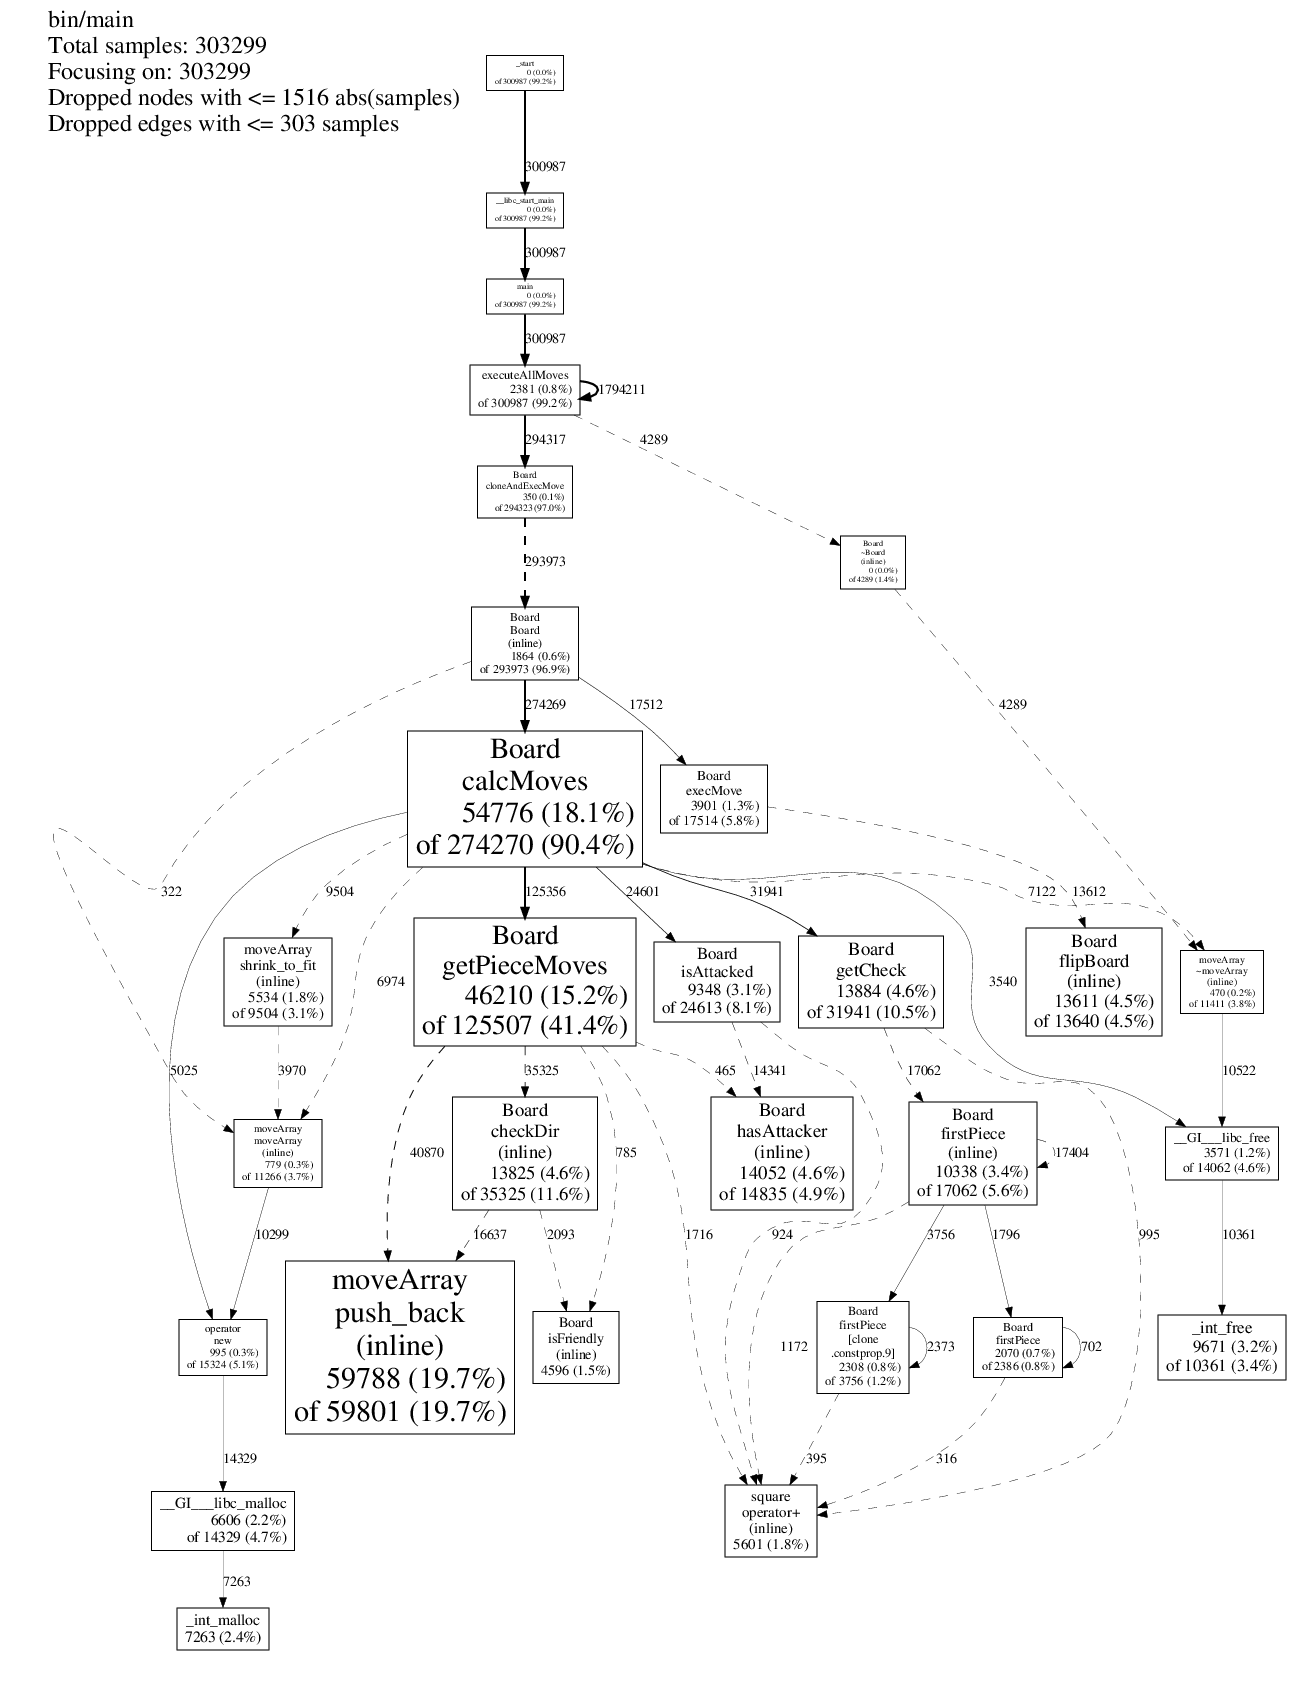
\includegraphics[width=8cm]{../../img/timing.png}}
\end{DoxyImageNoCaption}
 

\subsection{Constructor \& Destructor Documentation}
\index{Board@{Board}!Board@{Board}}
\index{Board@{Board}!Board@{Board}}
\subsubsection[{\texorpdfstring{Board(const Board \&other, const move mv)}{Board(const Board &other, const move mv)}}]{\setlength{\rightskip}{0pt plus 5cm}Board\+::\+Board (
\begin{DoxyParamCaption}
\item[{const {\bf Board} \&}]{other, }
\item[{const {\bf move}}]{mv}
\end{DoxyParamCaption}
)\hspace{0.3cm}{\ttfamily [private]}}\hypertarget{classBoard_a632d2e0f09a1ad6fe835dc11ef1238cc}{}\label{classBoard_a632d2e0f09a1ad6fe835dc11ef1238cc}


Private constructor to circumvent calculating the possible legal moves twice. 

This constructor is used when a move is executed. All the pieces must be copied, but copying all the legal moves is not necessary, as they are recalculated anyway. So, this private constructur is only to be used internally, when calling the {\itshape clone\+And\+Exec\+Move} function. 
\begin{DoxyParams}[1]{Parameters}
\mbox{\tt in}  & {\em other} & This is the board that is to be cloned. \\
\hline
\mbox{\tt in}  & {\em mv} & This is the move that is to be executed. \\
\hline
\end{DoxyParams}
\index{Board@{Board}!Board@{Board}}
\index{Board@{Board}!Board@{Board}}
\subsubsection[{\texorpdfstring{Board(const char $\ast$str, const bool file)}{Board(const char *str, const bool file)}}]{\setlength{\rightskip}{0pt plus 5cm}Board\+::\+Board (
\begin{DoxyParamCaption}
\item[{const char $\ast$}]{str, }
\item[{const bool}]{file}
\end{DoxyParamCaption}
)}\hypertarget{classBoard_a8dd2a85d6b43bcab4eaf83e1541aeb18}{}\label{classBoard_a8dd2a85d6b43bcab4eaf83e1541aeb18}


Read from F\+EN notation from file or string and calculate legal moves. 

\hyperlink{classBoard}{Board} constructor creating \hyperlink{classBoard}{Board} object from either a file or a string 
\begin{DoxyParams}[1]{Parameters}
\mbox{\tt in}  & {\em str} & Either the F\+EN string or the filename \\
\hline
\mbox{\tt in}  & {\em file} & Boolean whether to read file or string (true is file) \\
\hline
\end{DoxyParams}


\subsection{Member Function Documentation}
\index{Board@{Board}!calc\+Moves@{calc\+Moves}}
\index{calc\+Moves@{calc\+Moves}!Board@{Board}}
\subsubsection[{\texorpdfstring{calc\+Moves()}{calcMoves()}}]{\setlength{\rightskip}{0pt plus 5cm}void Board\+::calc\+Moves (
\begin{DoxyParamCaption}
{}
\end{DoxyParamCaption}
)\hspace{0.3cm}{\ttfamily [private]}}\hypertarget{classBoard_ad4d3ebb2342b74d9455a89924a54aa14}{}\label{classBoard_ad4d3ebb2342b74d9455a89924a54aa14}


Calculate legal moves. 

This function calculates all possible moves, and stores them in {\itshape legal\+Moves} member. Additionally, it updates the {\itshape check} flag, to indicate whether the player that is to move is check. Finally, it also updates the {\itshape draw} flag. If there are too few pieces on the board for any mate to occur, then this flag is set. \index{Board@{Board}!check\+Dir@{check\+Dir}}
\index{check\+Dir@{check\+Dir}!Board@{Board}}
\subsubsection[{\texorpdfstring{check\+Dir(move\+Array \&result, const check \&king\+Env, const square$<$ int $>$ base\+Pos, const square$<$ int $>$ dir) const }{checkDir(moveArray &result, const check &kingEnv, const square< int > basePos, const square< int > dir) const }}]{\setlength{\rightskip}{0pt plus 5cm}void Board\+::check\+Dir (
\begin{DoxyParamCaption}
\item[{{\bf move\+Array} \&}]{result, }
\item[{const {\bf check} \&}]{king\+Env, }
\item[{const {\bf square}$<$ int $>$}]{base\+Pos, }
\item[{const {\bf square}$<$ int $>$}]{dir}
\end{DoxyParamCaption}
) const\hspace{0.3cm}{\ttfamily [inline]}, {\ttfamily [private]}}\hypertarget{classBoard_af75103b55ce8129ffad6bc721162daa4}{}\label{classBoard_af75103b55ce8129ffad6bc721162daa4}


Check the possible moves of a piece along some file, rank or diagonal. 

This function helps the get\+Piece\+Moves function. It checks to which squares a long range piece (i.\+e. queen, rook or bishop) can move in a given direction, and appends these moves to the array of legal moves. 
\begin{DoxyParams}[1]{Parameters}
\mbox{\tt out}  & {\em result} & This is the array of moves which the found legal moves are appended to. \\
\hline
\mbox{\tt in}  & {\em king\+Env} & Through this {\itshape check} object, the information concerning whether a given move resolves check is supplied to the function. \\
\hline
\mbox{\tt in}  & {\em base\+Pos} & This is the position of the piece whose legal moves are investigated. \\
\hline
\mbox{\tt in}  & {\em dir} & This is the direction in which the legal moves are being checked. \\
\hline
\end{DoxyParams}
\index{Board@{Board}!clone\+And\+Exec\+Move@{clone\+And\+Exec\+Move}}
\index{clone\+And\+Exec\+Move@{clone\+And\+Exec\+Move}!Board@{Board}}
\subsubsection[{\texorpdfstring{clone\+And\+Exec\+Move(const move mv) const }{cloneAndExecMove(const move mv) const }}]{\setlength{\rightskip}{0pt plus 5cm}{\bf Board} Board\+::clone\+And\+Exec\+Move (
\begin{DoxyParamCaption}
\item[{const {\bf move}}]{mv}
\end{DoxyParamCaption}
) const}\hypertarget{classBoard_aef2523a362ab327fb628f4f226db52de}{}\label{classBoard_aef2523a362ab327fb628f4f226db52de}


Clone the current position and execute a move. 

Clone the board and execute the given move. Return the resulting position. 
\begin{DoxyParams}[1]{Parameters}
\mbox{\tt in}  & {\em mv} & The move to be executed. \\
\hline
\end{DoxyParams}
\begin{DoxyReturn}{Returns}
This function returns a new \hyperlink{classBoard}{Board} object, containing the new position, after the move was executed. 
\end{DoxyReturn}
\index{Board@{Board}!exec\+Move@{exec\+Move}}
\index{exec\+Move@{exec\+Move}!Board@{Board}}
\subsubsection[{\texorpdfstring{exec\+Move(const move mv)}{execMove(const move mv)}}]{\setlength{\rightskip}{0pt plus 5cm}void Board\+::exec\+Move (
\begin{DoxyParamCaption}
\item[{const {\bf move}}]{move}
\end{DoxyParamCaption}
)}\hypertarget{classBoard_a5732564ae8ce7f247072ded83f71dc75}{}\label{classBoard_a5732564ae8ce7f247072ded83f71dc75}


Execute a move. 

Execute a move on a given board and consequently flip the board and recalculate the legal moves. 
\begin{DoxyParams}[1]{Parameters}
\mbox{\tt in}  & {\em move} & This is the move that is to be executed. \\
\hline
\end{DoxyParams}
\index{Board@{Board}!first\+Piece@{first\+Piece}}
\index{first\+Piece@{first\+Piece}!Board@{Board}}
\subsubsection[{\texorpdfstring{first\+Piece(check \&result, const square$<$ int $>$ cur\+Pos, const square$<$ int $>$ dir, const int friendlies) const }{firstPiece(check &result, const square< int > curPos, const square< int > dir, const int friendlies) const }}]{\setlength{\rightskip}{0pt plus 5cm}bool Board\+::first\+Piece (
\begin{DoxyParamCaption}
\item[{{\bf check} \&}]{result, }
\item[{const {\bf square}$<$ int $>$}]{cur\+Pos, }
\item[{const {\bf square}$<$ int $>$}]{dir, }
\item[{const int}]{friendlies}
\end{DoxyParamCaption}
) const\hspace{0.3cm}{\ttfamily [private]}}\hypertarget{classBoard_a36298e9258372ab79f6b9fe7c6d68725}{}\label{classBoard_a36298e9258372ab79f6b9fe7c6d68725}


Investigate the possibility of attacks from dir to cur\+Pos (recursive) with heatmap. 

This function helps the get\+Check function to investigate the influence of one of the 8 directions on the output of the get\+Check function. 
\begin{DoxyParams}[1]{Parameters}
\mbox{\tt out}  & {\em result} & The check struct that get\+Check is working on. \\
\hline
\mbox{\tt in}  & {\em cur\+Pos} & The current position that is being investigated. \\
\hline
\mbox{\tt in}  & {\em dir} & The direction in which is being checked whether there are attacks going on. \\
\hline
\mbox{\tt in}  & {\em friendlies} & This value determines the number of friendly pieces that were already encountered. If this is 1, and an attacking piece is encountered, then {\itshape result} will indicate that this piece is pinned. \\
\hline
\end{DoxyParams}
\begin{DoxyReturn}{Returns}
This function returns a boolean. True is returned, if the square indicated by {\itshape cur\+Pos} is under attack from the direction indicated by {\itshape dir}. Otherwise, false is returned. 
\end{DoxyReturn}
\index{Board@{Board}!flip\+Board@{flip\+Board}}
\index{flip\+Board@{flip\+Board}!Board@{Board}}
\subsubsection[{\texorpdfstring{flip\+Board()}{flipBoard()}}]{\setlength{\rightskip}{0pt plus 5cm}void Board\+::flip\+Board (
\begin{DoxyParamCaption}
{}
\end{DoxyParamCaption}
)\hspace{0.3cm}{\ttfamily [private]}}\hypertarget{classBoard_aeea5a9ddcdeb6e4c087f53e71f6c11ec}{}\label{classBoard_aeea5a9ddcdeb6e4c087f53e71f6c11ec}


Flip the board such that pawns always advance in the direction of increasing rank. 

This function flips the board. More precisely, it mirrors the position of all pieces along the axis between the 4th and 5th rank. So, for example, a piece on e3 is placed on e6, and a piece on a8 is placed on a1. This function is used to ensure that the player that is to move always plays with its pawns advancing to ever higher ranks. \index{Board@{Board}!from\+File@{from\+File}}
\index{from\+File@{from\+File}!Board@{Board}}
\subsubsection[{\texorpdfstring{from\+File(const char $\ast$file\+Name)}{fromFile(const char *fileName)}}]{\setlength{\rightskip}{0pt plus 5cm}int Board\+::from\+File (
\begin{DoxyParamCaption}
\item[{const char $\ast$}]{file\+Name}
\end{DoxyParamCaption}
)\hspace{0.3cm}{\ttfamily [private]}}\hypertarget{classBoard_a4043087fc35e9706d0e83ec07225fe33}{}\label{classBoard_a4043087fc35e9706d0e83ec07225fe33}


Read the F\+EN notation from a file. 

Initialize a \hyperlink{classBoard}{Board} object from a file containing a string in F\+EN notation. 
\begin{DoxyParams}{Parameters}
{\em file\+Name} & The name of the file. \\
\hline
\end{DoxyParams}
\begin{DoxyReturn}{Returns}
This function returns an error code, according to the following table\+: \tabulinesep=1mm
\begin{longtabu} spread 0pt [c]{*2{|X[-1]}|}
\hline
\rowcolor{\tableheadbgcolor}\PBS\raggedleft {\bf Code }&{\bf Description  }\\\cline{1-2}
\endfirsthead
\hline
\endfoot
\hline
\rowcolor{\tableheadbgcolor}\PBS\raggedleft {\bf Code }&{\bf Description  }\\\cline{1-2}
\endhead
\PBS\raggedleft 0 &Success. \\\cline{1-2}
\PBS\raggedleft 1 &The syntax of str is wrong. \\\cline{1-2}
\end{longtabu}

\end{DoxyReturn}
\index{Board@{Board}!from\+Str@{from\+Str}}
\index{from\+Str@{from\+Str}!Board@{Board}}
\subsubsection[{\texorpdfstring{from\+Str(const char $\ast$str)}{fromStr(const char *str)}}]{\setlength{\rightskip}{0pt plus 5cm}int Board\+::from\+Str (
\begin{DoxyParamCaption}
\item[{const char $\ast$}]{str}
\end{DoxyParamCaption}
)\hspace{0.3cm}{\ttfamily [private]}}\hypertarget{classBoard_a49045c77d568e4b5a00f176a2add54c8}{}\label{classBoard_a49045c77d568e4b5a00f176a2add54c8}


Read the F\+EN notation from a string. 

Initialize a \hyperlink{classBoard}{Board} object from a string in F\+EN notation. 
\begin{DoxyParams}[1]{Parameters}
\mbox{\tt in}  & {\em str} & The string in F\+EN notation \\
\hline
\end{DoxyParams}
\begin{DoxyReturn}{Returns}
This function returns an error code, according to the following table\+: \tabulinesep=1mm
\begin{longtabu} spread 0pt [c]{*2{|X[-1]}|}
\hline
\rowcolor{\tableheadbgcolor}\PBS\raggedleft {\bf Code }&{\bf Description  }\\\cline{1-2}
\endfirsthead
\hline
\endfoot
\hline
\rowcolor{\tableheadbgcolor}\PBS\raggedleft {\bf Code }&{\bf Description  }\\\cline{1-2}
\endhead
\PBS\raggedleft 0 &Success. \\\cline{1-2}
\PBS\raggedleft 1 &The syntax of str is wrong. \\\cline{1-2}
\end{longtabu}

\end{DoxyReturn}
\index{Board@{Board}!get\+Check@{get\+Check}}
\index{get\+Check@{get\+Check}!Board@{Board}}
\subsubsection[{\texorpdfstring{get\+Check(const square$<$ int $>$ king\+Pos)}{getCheck(const square< int > kingPos)}}]{\setlength{\rightskip}{0pt plus 5cm}{\bf check} Board\+::get\+Check (
\begin{DoxyParamCaption}
\item[{const {\bf square}$<$ int $>$}]{king\+Pos}
\end{DoxyParamCaption}
)\hspace{0.3cm}{\ttfamily [private]}}\hypertarget{classBoard_afc291baf2c205a64255e8e55ffeff004}{}\label{classBoard_afc291baf2c205a64255e8e55ffeff004}


Get the details about a possible check at king\+Pos. 

This function finds out what is going on in relation to the king of the player that is to move. In particular, it returns a check struct containing information about pinned pieces and squares that can resolve check. Moreover, it updates the check flag. 
\begin{DoxyParams}[1]{Parameters}
\mbox{\tt in}  & {\em king\+Pos} & The position of the king. \\
\hline
\end{DoxyParams}
\begin{DoxyReturn}{Returns}
This function returns a check object, containing information about pinned pieces and, in case of check, how many pieces are attacking the king, and, in case of 1 attacking piece, which squares will resolve the check. 
\end{DoxyReturn}
\index{Board@{Board}!get\+Piece\+Moves@{get\+Piece\+Moves}}
\index{get\+Piece\+Moves@{get\+Piece\+Moves}!Board@{Board}}
\subsubsection[{\texorpdfstring{get\+Piece\+Moves(move\+Array \&result, const check \&king\+Env, const square$<$ int $>$ cur\+Pos, const square$<$ int $>$ king\+Pos)}{getPieceMoves(moveArray &result, const check &kingEnv, const square< int > curPos, const square< int > kingPos)}}]{\setlength{\rightskip}{0pt plus 5cm}void Board\+::get\+Piece\+Moves (
\begin{DoxyParamCaption}
\item[{{\bf move\+Array} \&}]{result, }
\item[{const {\bf check} \&}]{king\+Env, }
\item[{const {\bf square}$<$ int $>$}]{cur\+Pos, }
\item[{const {\bf square}$<$ int $>$}]{king\+Pos}
\end{DoxyParamCaption}
)\hspace{0.3cm}{\ttfamily [private]}}\hypertarget{classBoard_aa70526dde51ab18ec4011c07a7e38e60}{}\label{classBoard_aa70526dde51ab18ec4011c07a7e38e60}


Calculate the legal moves of the piece on square$<$int$>$ cur\+Pos. 

This function helps the calc\+Moves function. It investigates the legal moves that one particular piece can make, and appends these to the temporary moves array created by calc\+Moves. 
\begin{DoxyParams}[1]{Parameters}
\mbox{\tt out}  & {\em result} & This is the array that the newly found moves are being appended to. \\
\hline
\mbox{\tt in}  & {\em king\+Env} & The function uses this data structure to check whether the piece is pinned, or helps resolving a check. \\
\hline
\mbox{\tt in}  & {\em cur\+Pos} & This is the square where the piece, whose legal moves are begin investigated, is located. \\
\hline
\mbox{\tt in}  & {\em king\+Pos} & This is the square where the king of the player who is to move is located. Its value is used to speed up special cases of taking en passant. \\
\hline
\end{DoxyParams}
\index{Board@{Board}!has\+Attacker@{has\+Attacker}}
\index{has\+Attacker@{has\+Attacker}!Board@{Board}}
\subsubsection[{\texorpdfstring{has\+Attacker(square$<$ int $>$ pos, const square$<$ int $>$ dir) const }{hasAttacker(square< int > pos, const square< int > dir) const }}]{\setlength{\rightskip}{0pt plus 5cm}bool Board\+::has\+Attacker (
\begin{DoxyParamCaption}
\item[{{\bf square}$<$ int $>$}]{pos, }
\item[{const {\bf square}$<$ int $>$}]{dir}
\end{DoxyParamCaption}
) const\hspace{0.3cm}{\ttfamily [private]}}\hypertarget{classBoard_ab3a977ba17a7e6d6b669777566165b35}{}\label{classBoard_ab3a977ba17a7e6d6b669777566165b35}


Invesitgate the possibility of attacks from dir at cur\+Pos. 

This function helps the is\+Attacked function to determine whether an attack over a long distance from a fixed direction occurs. 
\begin{DoxyParams}[1]{Parameters}
\mbox{\tt in}  & {\em pos} & The position of which is determined whether it is under attack. \\
\hline
\mbox{\tt in}  & {\em dir} & The direction in which is being checked whether there is an attacker. \\
\hline
\end{DoxyParams}
\begin{DoxyReturn}{Returns}
This function returns a boolean, indicating whether there is an emeny piece attacking the square {\itshape pos} from direction {\itshape dir}. 
\end{DoxyReturn}
\index{Board@{Board}!print\+Board@{print\+Board}}
\index{print\+Board@{print\+Board}!Board@{Board}}
\subsubsection[{\texorpdfstring{print\+Board() const }{printBoard() const }}]{\setlength{\rightskip}{0pt plus 5cm}void Board\+::print\+Board (
\begin{DoxyParamCaption}
{}
\end{DoxyParamCaption}
) const}\hypertarget{classBoard_a58b38efec8c8ce21b55546da09685a3e}{}\label{classBoard_a58b38efec8c8ce21b55546da09685a3e}


Print a formatted representation of the board. 

Give a nice overview of the current position in the terminal window 

\subsection{Member Data Documentation}
\index{Board@{Board}!board@{board}}
\index{board@{board}!Board@{Board}}
\subsubsection[{\texorpdfstring{board}{board}}]{\setlength{\rightskip}{0pt plus 5cm}{\bf Piece\+::\+Piece} Board\+::board\mbox{[}8\mbox{]}\mbox{[}8\mbox{]}\hspace{0.3cm}{\ttfamily [private]}}\hypertarget{classBoard_acdbd7620b4c8bc08b2e42623c2a12a39}{}\label{classBoard_acdbd7620b4c8bc08b2e42623c2a12a39}
This character array stores the position of the pieces on the board. Every entry in the character array corresponds to one square. The values of these characters correspond to the widely used F\+EN notation. \tabulinesep=1mm
\begin{longtabu} spread 0pt [c]{*3{|X[-1]}|}
\hline
\rowcolor{\tableheadbgcolor}{\bf Value }&{\bf A\+S\+C\+II representation }&{\bf \hyperlink{namespacePiece}{Piece}  }\\\cline{1-3}
\endfirsthead
\hline
\endfoot
\hline
\rowcolor{\tableheadbgcolor}{\bf Value }&{\bf A\+S\+C\+II representation }&{\bf \hyperlink{namespacePiece}{Piece}  }\\\cline{1-3}
\endhead
0x20 &Space &None \\\cline{1-3}
0x4B &K &White king \\\cline{1-3}
0x51 &Q &White queen \\\cline{1-3}
0x52 &R &White rook \\\cline{1-3}
0x42 &B &White bishop \\\cline{1-3}
0x4E &N &White knight \\\cline{1-3}
0x50 &P &White pawn \\\cline{1-3}
0x6B &k &Black king \\\cline{1-3}
0x71 &q &Black queen \\\cline{1-3}
0x72 &r &Black rook \\\cline{1-3}
0x62 &b &Black bishop \\\cline{1-3}
0x6E &n &Black knight \\\cline{1-3}
0x70 &p &Black pawn \\\cline{1-3}
\end{longtabu}
A convenient feature of this notation is that determining whether a piece is black can be done by doing an A\+ND operation with the bitmask 0x20. \index{Board@{Board}!en\+Passant@{en\+Passant}}
\index{en\+Passant@{en\+Passant}!Board@{Board}}
\subsubsection[{\texorpdfstring{en\+Passant}{enPassant}}]{\setlength{\rightskip}{0pt plus 5cm}signed char Board\+::en\+Passant\hspace{0.3cm}{\ttfamily [private]}}\hypertarget{classBoard_aad3145585c03f739311c35fa8f3277d3}{}\label{classBoard_aad3145585c03f739311c35fa8f3277d3}
This signed character stores whether the opponent in the last move advanced one of his pawns by two squares. If he did not, then the value is -\/1. Otherwise, it is in the range 0-\/7, where the value corresponds to the file on which the pawn was advanced in the last move. \index{Board@{Board}!legal\+Moves@{legal\+Moves}}
\index{legal\+Moves@{legal\+Moves}!Board@{Board}}
\subsubsection[{\texorpdfstring{legal\+Moves}{legalMoves}}]{\setlength{\rightskip}{0pt plus 5cm}{\bf move\+Array} Board\+::legal\+Moves\hspace{0.3cm}{\ttfamily [private]}}\hypertarget{classBoard_aaf6a2575c3bc280ddc9e445efd213e14}{}\label{classBoard_aaf6a2575c3bc280ddc9e445efd213e14}
Here, all the legal moves that the player to move can play are stored. We have chosen not to go with the std\+::vector$<$move$>$ implementation, as our custom implementation saves about 15\% of runtime. \index{Board@{Board}!state@{state}}
\index{state@{state}!Board@{Board}}
\subsubsection[{\texorpdfstring{state}{state}}]{\setlength{\rightskip}{0pt plus 5cm}char Board\+::state\hspace{0.3cm}{\ttfamily [private]}}\hypertarget{classBoard_a46a6e23b1b18542b10938f2b333862f1}{}\label{classBoard_a46a6e23b1b18542b10938f2b333862f1}
This character contains seven flags. These flags store some auxiliary information about the position. They are listed in the table below. \tabulinesep=1mm
\begin{longtabu} spread 0pt [c]{*3{|X[-1]}|}
\hline
\rowcolor{\tableheadbgcolor}{\bf Bit }&{\bf Keyword }&{\bf Description  }\\\cline{1-3}
\endfirsthead
\hline
\endfoot
\hline
\rowcolor{\tableheadbgcolor}{\bf Bit }&{\bf Keyword }&{\bf Description  }\\\cline{1-3}
\endhead
0 &check\+Mask &This flag is set if the player to move is checked. \\\cline{1-3}
1 &white\+Castle\+Kingside\+Mask &This flag is set if the player to move has not yet moved his king and kingside rook. \\\cline{1-3}
2 &white\+Castle\+Queenside\+Mask &This flag is set if the player to move has not yet moved his king and queenside rook. \\\cline{1-3}
3 &black\+Castle\+Kingside\+Mask &This flag is set if the player that is not to move has not yet moved his king and kingside rook. \\\cline{1-3}
4 &black\+Castle\+Queenside\+Mask &This flag is set if the player that is not to move has not yet moved his king and queenside rook. \\\cline{1-3}
5 &black\+To\+Move\+Mask &This flag is set if black currently is to move. \\\cline{1-3}
6 &draw\+Mask &This flag is set if there is a stalemate, or if giving checkmate with the pieces that are left on the board is not possible. In both cases, the game is considered to be drawn. \\\cline{1-3}
\end{longtabu}
Notice that it is no coincidence that the black\+To\+Move\+Mask corresponds to the fifth bit. The fifth bit being set in a character yields 0x20, which is exactly the mask that can be used to determine whether a piece is black or white. 

The documentation for this class was generated from the following files\+:\begin{DoxyCompactItemize}
\item 
src/Board.\+h\item 
src/Board.\+cpp\end{DoxyCompactItemize}

\hypertarget{structcheck}{}\section{check Struct Reference}
\label{structcheck}\index{check@{check}}


{\ttfamily \#include $<$Board.\+h$>$}

\subsection*{Public Attributes}
\begin{DoxyCompactItemize}
\item 
\mbox{\Hypertarget{structcheck_a004e9a83f3635e9ec1e40c98d3ba0519}\label{structcheck_a004e9a83f3635e9ec1e40c98d3ba0519}} 
int \hyperlink{structcheck_a004e9a83f3635e9ec1e40c98d3ba0519}{len}
\begin{DoxyCompactList}\small\item\em The number of pieces attacking the king. \end{DoxyCompactList}\item 
char \hyperlink{structcheck_a20edc7f43122fbfd399629ed8b41dc6a}{heat\+Map} \mbox{[}8\mbox{]}\mbox{[}8\mbox{]}
\end{DoxyCompactItemize}


\subsection{Detailed Description}
The check struct stores all the information that is somewhat related to the king, and is used for internal communication within the {\itshape calc\+Moves} method only. On the one hand, it stores the number of pieces that are giving check to the king, and if the king is checked, which squares can be used to resolve this check. Furthermore, it stores whether a piece is pinned, and if so, in which direction. 

\subsection{Member Data Documentation}
\mbox{\Hypertarget{structcheck_a20edc7f43122fbfd399629ed8b41dc6a}\label{structcheck_a20edc7f43122fbfd399629ed8b41dc6a}} 
\index{check@{check}!heat\+Map@{heat\+Map}}
\index{heat\+Map@{heat\+Map}!check@{check}}
\subsubsection{\texorpdfstring{heat\+Map}{heatMap}}
{\footnotesize\ttfamily char check\+::heat\+Map\mbox{[}8\mbox{]}\mbox{[}8\mbox{]}}

All the 64 character entries of the heatmap correspond to exactly one square on the chess board. The encoding of the heatmap depends on the piece that is occupying the square. The table below lists all the cases. \tabulinesep=1mm
\begin{longtabu} spread 0pt [c]{*{3}{|X[-1]}|}
\hline
\rowcolor{\tableheadbgcolor}\textbf{ Occupation of the square }&\textbf{ Value }&\textbf{ Description }\\\cline{1-3}
\endfirsthead
\hline
\endfoot
\hline
\rowcolor{\tableheadbgcolor}\textbf{ Occupation of the square }&\textbf{ Value }&\textbf{ Description }\\\cline{1-3}
\endhead
\multirow{2}{\linewidth}{Empty }&0 &No peculiarities. \\\cline{2-3}
&1 &Placing a friendly piece here will resolve check. \\\cline{1-3}
\multirow{2}{\linewidth}{Enemy piece }&0 &No peculiarities. \\\cline{2-3}
&1 &Taking this piece will resolve check. \\\cline{1-3}
\multirow{5}{\linewidth}{Friendly piece }&0 &No peculiarities. \\\cline{2-3}
&1 &This piece is pinned, such that it can only move in the northwest-\/southeast direction. \\\cline{2-3}
&2 &This piece is pinned, such that it can only move in the horizontal direction. \\\cline{2-3}
&3 &This piece is pinned, such that it can only move in the northeast-\/southwest direction. \\\cline{2-3}
&4 &This piece is pinned, such that it can only move in the vertical direction. \\\cline{1-3}
\end{longtabu}
Some edge cases are not included in the check structure. For example, consider the following board\+:  
\begin{DoxyImageNoCaption}
  \mbox{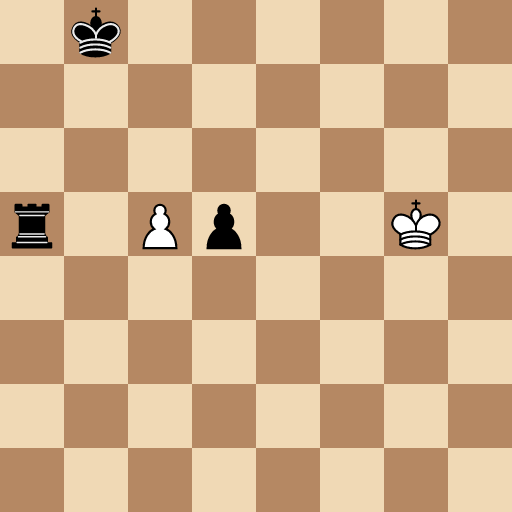
\includegraphics[width=4cm]{../../img/EnPassantPin.png}}
\end{DoxyImageNoCaption}
 If white now decides to take the black pawn en passant, then white checks himself, so this is not a legal move. Yet the white pawn is not considered to be pinned, as it can advance without checking anyone. This, then, is a situation that cannot be stored in the check struct, and needs to be handled separately. 

The documentation for this struct was generated from the following file\+:\begin{DoxyCompactItemize}
\item 
src/Board.\+h\end{DoxyCompactItemize}

\hypertarget{classDFS}{}\section{D\+FS Class Reference}
\label{classDFS}\index{D\+FS@{D\+FS}}


{\ttfamily \#include $<$D\+F\+S.\+h$>$}

\subsection*{Public Member Functions}
\begin{DoxyCompactItemize}
\item 
\hyperlink{classDFS_a8db913929c53b5cba8f145c281ef99f8}{D\+FS} (\hyperlink{classBoard}{Board} $\ast$\+\_\+start, unsigned int \+\_\+max\+Depth, bool \+\_\+turbo)
\begin{DoxyCompactList}\small\item\em The constructor. \end{DoxyCompactList}\item 
\hyperlink{classDFS_ac8748bddd420ae23a10620cb4b5714c5}{D\+FS} (\hyperlink{classBoard}{Board} $\ast$\+\_\+start)\hypertarget{classDFS_ac8748bddd420ae23a10620cb4b5714c5}{}\label{classDFS_ac8748bddd420ae23a10620cb4b5714c5}

\begin{DoxyCompactList}\small\item\em Default constructor, using the default values. \end{DoxyCompactList}\item 
\hyperlink{structDFSresult}{D\+F\+Sresult} \hyperlink{classDFS_a49982f77146f1839b15a36c6974e43d1}{search} ()
\end{DoxyCompactItemize}
\subsection*{Private Member Functions}
\begin{DoxyCompactItemize}
\item 
{\footnotesize template$<$bool T$>$ }\\\hyperlink{structDFSresult}{D\+F\+Sresult} \hyperlink{classDFS_a8b4c8f013eb056faee52530deb5a9971}{best\+\_\+outcome} (\hyperlink{classBoard}{Board}, unsigned int)
\end{DoxyCompactItemize}
\subsection*{Private Attributes}
\begin{DoxyCompactItemize}
\item 
unsigned int \hyperlink{classDFS_aacbeeaf0eebb3a37ad25b0c42bd27e64}{max\+Depth}\hypertarget{classDFS_aacbeeaf0eebb3a37ad25b0c42bd27e64}{}\label{classDFS_aacbeeaf0eebb3a37ad25b0c42bd27e64}

\begin{DoxyCompactList}\small\item\em The maximum number of half-\/moves to be executed from the initial position. \end{DoxyCompactList}\item 
unsigned int \hyperlink{classDFS_a17abe1c016f7efe83c51c4ee9ba541f3}{cur\+Depth}\hypertarget{classDFS_a17abe1c016f7efe83c51c4ee9ba541f3}{}\label{classDFS_a17abe1c016f7efe83c51c4ee9ba541f3}

\begin{DoxyCompactList}\small\item\em The number of half-\/moves at which the current branches that are under investigation are being pruned. \end{DoxyCompactList}\item 
\hyperlink{classBoard}{Board} $\ast$ \hyperlink{classDFS_a34ffac99b64c8f83889e66d47fa94787}{start}\hypertarget{classDFS_a34ffac99b64c8f83889e66d47fa94787}{}\label{classDFS_a34ffac99b64c8f83889e66d47fa94787}

\begin{DoxyCompactList}\small\item\em A pointer to the \hyperlink{classBoard}{Board} object storing the initial position. \end{DoxyCompactList}\item 
bool \hyperlink{classDFS_a3c4278e719f9a1d9766b4d5c60548137}{turbo}\hypertarget{classDFS_a3c4278e719f9a1d9766b4d5c60548137}{}\label{classDFS_a3c4278e719f9a1d9766b4d5c60548137}

\begin{DoxyCompactList}\small\item\em A boolean variable storing whether the search should be conducted using turbo mode, affecting the behavior of the best\+\_\+outcome method. \end{DoxyCompactList}\end{DoxyCompactItemize}


\subsection{Detailed Description}
The \hyperlink{classDFS}{D\+FS} class performs the Depth First Search through all the possible positions. It allows two possible search modes. One is the standard mode of search. It searches through the entire tree of possible game continuations with a given depth, and returns the best move sequence of all these continuations. The other is referred to as the turbo mode. This mode is aimed at finding checkmates for the player that initially is to move. Using this mode, the algorithm will correctly find forced mate sequences, if they exist, but in other cases it might not identify the best game continuation for the opponent. 

\subsection{Constructor \& Destructor Documentation}
\index{D\+FS@{D\+FS}!D\+FS@{D\+FS}}
\index{D\+FS@{D\+FS}!D\+FS@{D\+FS}}
\subsubsection[{\texorpdfstring{D\+F\+S(\+Board $\ast$\+\_\+start, unsigned int \+\_\+max\+Depth, bool \+\_\+turbo)}{DFS(Board *_start, unsigned int _maxDepth, bool _turbo)}}]{\setlength{\rightskip}{0pt plus 5cm}D\+F\+S\+::\+D\+FS (
\begin{DoxyParamCaption}
\item[{{\bf Board} $\ast$}]{\+\_\+start, }
\item[{unsigned int}]{\+\_\+max\+Depth, }
\item[{bool}]{\+\_\+turbo}
\end{DoxyParamCaption}
)}\hypertarget{classDFS_a8db913929c53b5cba8f145c281ef99f8}{}\label{classDFS_a8db913929c53b5cba8f145c281ef99f8}


The constructor. 

\hyperlink{classDFS}{D\+FS} or depth first search constructor. 
\begin{DoxyParams}[1]{Parameters}
\mbox{\tt in}  & {\em \+\_\+start} & Starting board pointer \\
\hline
\mbox{\tt in}  & {\em \+\_\+max\+Depth} & Maximal depth to search. \\
\hline
\mbox{\tt in}  & {\em \+\_\+turbo} & Turbo mode. \\
\hline
\end{DoxyParams}


\subsection{Member Function Documentation}
\index{D\+FS@{D\+FS}!best\+\_\+outcome@{best\+\_\+outcome}}
\index{best\+\_\+outcome@{best\+\_\+outcome}!D\+FS@{D\+FS}}
\subsubsection[{\texorpdfstring{best\+\_\+outcome(\+Board, unsigned int)}{best_outcome(Board, unsigned int)}}]{\setlength{\rightskip}{0pt plus 5cm}template$<$bool T$>$ {\bf D\+F\+Sresult} D\+F\+S\+::best\+\_\+outcome (
\begin{DoxyParamCaption}
\item[{{\bf Board}}]{board, }
\item[{unsigned int}]{depth}
\end{DoxyParamCaption}
)\hspace{0.3cm}{\ttfamily [private]}}\hypertarget{classDFS_a8b4c8f013eb056faee52530deb5a9971}{}\label{classDFS_a8b4c8f013eb056faee52530deb5a9971}
Calculate what the best outcome is for a single node. First of all, it is checked whether the current position is a mate or a draw. If this is the case, this is reported to the calling function. Next, all the moves that are possible in the position are investigated one by one. For every move, it is returned to this function whether it results in a win, loss, draw, or an undecided position, and how many moves it takes. This function, then, chooses the best option among all of these moves, and returns that to the calling function. In turbo mode, at odd depths of search (so when the opponent is to move), not necessarily the best move is returned, but just a move that avoids being checkmated, whenever possible. 
\begin{DoxyParams}[1]{Parameters}
\mbox{\tt in}  & {\em board} & The board to consider \\
\hline
\mbox{\tt in}  & {\em depth} & The current depth \\
\hline
\end{DoxyParams}
\begin{DoxyReturn}{Returns}
This function returns a \hyperlink{structDFSresult}{D\+F\+Sresult} object containing the best state possible of the previous node the depth at which the state occurred and the moves leading to that state from this node. 
\end{DoxyReturn}
\index{D\+FS@{D\+FS}!search@{search}}
\index{search@{search}!D\+FS@{D\+FS}}
\subsubsection[{\texorpdfstring{search()}{search()}}]{\setlength{\rightskip}{0pt plus 5cm}{\bf D\+F\+Sresult} D\+F\+S\+::search (
\begin{DoxyParamCaption}
{}
\end{DoxyParamCaption}
)}\hypertarget{classDFS_a49982f77146f1839b15a36c6974e43d1}{}\label{classDFS_a49982f77146f1839b15a36c6974e43d1}
Do the actual search. The search is conducted as follows. First of all, all the possible moves are investigated with depth 1. If this does not yield a decisive result, then the depth at which is searched is increased by 2. This is done until the maximum depth is reached. Increasing the depth like this does not increase the total time complexity of the program, and is therefore perfectly suitable for obtaining preliminary results without having to conduct the entire search, while not giving rise to unacceptable amounts of overhead. Only at the maximum depth level, progress reports are being shown. \begin{DoxyReturn}{Returns}
This function returns a \hyperlink{structDFSresult}{D\+F\+Sresult} object containing the best state possible from the start board the worstcase depth at which the state occurred and the moves leading to that state from the position. 
\end{DoxyReturn}


The documentation for this class was generated from the following files\+:\begin{DoxyCompactItemize}
\item 
src/D\+F\+S.\+h\item 
src/D\+F\+S.\+cpp\end{DoxyCompactItemize}

\hypertarget{structDFSresult}{}\section{D\+F\+Sresult Struct Reference}
\label{structDFSresult}\index{D\+F\+Sresult@{D\+F\+Sresult}}


{\ttfamily \#include $<$D\+F\+S.\+h$>$}

\subsection*{Public Attributes}
\begin{DoxyCompactItemize}
\item 
int \hyperlink{structDFSresult_a05517437c3e1db1f5b212f2862801b85}{state}
\item 
unsigned int \hyperlink{structDFSresult_a0d91b41c51df56f42e450f9ce82fa4f2}{depth}
\item 
std\+::stack$<$ \hyperlink{structmove}{move} $>$ \hyperlink{structDFSresult_acbab901f87df79e0ff718f4fd9435a0f}{moves}
\end{DoxyCompactItemize}


\subsection{Detailed Description}
The \hyperlink{structDFSresult}{D\+F\+Sresult} structure contains the result of the Depth First Search. It stores whether the given position is a win, a loss, a draw, or undecided, and it contains the move sequence the search routine considered best. 

\subsection{Member Data Documentation}
\mbox{\Hypertarget{structDFSresult_a0d91b41c51df56f42e450f9ce82fa4f2}\label{structDFSresult_a0d91b41c51df56f42e450f9ce82fa4f2}} 
\index{D\+F\+Sresult@{D\+F\+Sresult}!depth@{depth}}
\index{depth@{depth}!D\+F\+Sresult@{D\+F\+Sresult}}
\subsubsection{\texorpdfstring{depth}{depth}}
{\footnotesize\ttfamily unsigned int D\+F\+Sresult\+::depth}

The member variable depth stores the length of the resulting stack, so it equals the number of half-\/moves that the stack contains. \mbox{\Hypertarget{structDFSresult_acbab901f87df79e0ff718f4fd9435a0f}\label{structDFSresult_acbab901f87df79e0ff718f4fd9435a0f}} 
\index{D\+F\+Sresult@{D\+F\+Sresult}!moves@{moves}}
\index{moves@{moves}!D\+F\+Sresult@{D\+F\+Sresult}}
\subsubsection{\texorpdfstring{moves}{moves}}
{\footnotesize\ttfamily std\+::stack$<$\hyperlink{structmove}{move}$>$ D\+F\+Sresult\+::moves}

The member variable moves stores the best move sequence that the search algorithm came up with. It uses the std\+::stack implementation. \mbox{\Hypertarget{structDFSresult_a05517437c3e1db1f5b212f2862801b85}\label{structDFSresult_a05517437c3e1db1f5b212f2862801b85}} 
\index{D\+F\+Sresult@{D\+F\+Sresult}!state@{state}}
\index{state@{state}!D\+F\+Sresult@{D\+F\+Sresult}}
\subsubsection{\texorpdfstring{state}{state}}
{\footnotesize\ttfamily int D\+F\+Sresult\+::state}

This is the return state of the search routine. It is encoded as follows. \tabulinesep=1mm
\begin{longtabu} spread 0pt [c]{*{2}{|X[-1]}|}
\hline
\rowcolor{\tableheadbgcolor}\textbf{ Value }&\textbf{ Description  }\\\cline{1-2}
\endfirsthead
\hline
\endfoot
\hline
\rowcolor{\tableheadbgcolor}\textbf{ Value }&\textbf{ Description  }\\\cline{1-2}
\endhead
-\/2 &The position is winning for the player that currently is to move, provided that he plays correctly. \\\cline{1-2}
0 &The position is a draw. \\\cline{1-2}
1 &The position is still undecided. There is no forced mate possible within the number of moves that the search algorithm used as its maximum depth. \\\cline{1-2}
2 &The position is losing for the player that currently is to move, provided that the opponent plays correctly. \\\cline{1-2}
\end{longtabu}


The documentation for this struct was generated from the following file\+:\begin{DoxyCompactItemize}
\item 
src/D\+F\+S.\+h\end{DoxyCompactItemize}

\hypertarget{structmove}{}\section{move Struct Reference}
\label{structmove}\index{move@{move}}
\subsection*{Public Member Functions}
\begin{DoxyCompactItemize}
\item 
\mbox{\Hypertarget{structmove_a1586ed1c5f7173c4b60fa306522e4f64}\label{structmove_a1586ed1c5f7173c4b60fa306522e4f64}} 
void {\bfseries print\+Move} (bool black\+To\+Move)
\end{DoxyCompactItemize}
\subsection*{Public Attributes}
\begin{DoxyCompactItemize}
\item 
\mbox{\Hypertarget{structmove_a3f8a82f7c7bc55f55874026ac254cd85}\label{structmove_a3f8a82f7c7bc55f55874026ac254cd85}} 
\hyperlink{structsquare}{square}$<$ void $>$ {\bfseries start}
\item 
\mbox{\Hypertarget{structmove_a205ae16ec975ed71eb4233bb38d21a75}\label{structmove_a205ae16ec975ed71eb4233bb38d21a75}} 
\hyperlink{structsquare}{square}$<$ void $>$ {\bfseries end}
\item 
\mbox{\Hypertarget{structmove_a87fc4fc521c961cce03613dcb6cd0c6b}\label{structmove_a87fc4fc521c961cce03613dcb6cd0c6b}} 
Piece\+::\+Piece {\bfseries promote\+To}
\end{DoxyCompactItemize}


The documentation for this struct was generated from the following file\+:\begin{DoxyCompactItemize}
\item 
src/Move.\+h\end{DoxyCompactItemize}

\hypertarget{structmoveArray}{}\section{move\+Array Struct Reference}
\label{structmoveArray}\index{move\+Array@{move\+Array}}


{\ttfamily \#include $<$Move\+Array.\+h$>$}

\subsection*{Public Member Functions}
\begin{DoxyCompactItemize}
\item 
\hyperlink{structmoveArray_adad62027e18e94b8034a5162a161e979}{move\+Array} ()\hypertarget{structmoveArray_adad62027e18e94b8034a5162a161e979}{}\label{structmoveArray_adad62027e18e94b8034a5162a161e979}

\begin{DoxyCompactList}\small\item\em The default constructor. \end{DoxyCompactList}\item 
\hyperlink{structmoveArray_a3cb7e6bc3daac07f3005e7ca18af4589}{move\+Array} (const int n)\hypertarget{structmoveArray_a3cb7e6bc3daac07f3005e7ca18af4589}{}\label{structmoveArray_a3cb7e6bc3daac07f3005e7ca18af4589}

\begin{DoxyCompactList}\small\item\em A constructor reserving space for {\itshape n} moves. \end{DoxyCompactList}\item 
\hyperlink{structmoveArray_a78117ae0946c2a61ff86a832c420c854}{move\+Array} (const \hyperlink{structmoveArray}{move\+Array} \&other)\hypertarget{structmoveArray_a78117ae0946c2a61ff86a832c420c854}{}\label{structmoveArray_a78117ae0946c2a61ff86a832c420c854}

\begin{DoxyCompactList}\small\item\em The copy constructor. \end{DoxyCompactList}\item 
\hyperlink{structmoveArray_ac0a694dea63dc46f9c524766aa457d4f}{$\sim$move\+Array} ()\hypertarget{structmoveArray_ac0a694dea63dc46f9c524766aa457d4f}{}\label{structmoveArray_ac0a694dea63dc46f9c524766aa457d4f}

\begin{DoxyCompactList}\small\item\em The destructor. \end{DoxyCompactList}\item 
\hyperlink{structmoveArray}{move\+Array} \& \hyperlink{structmoveArray_ad7c5f1a65aab09aebbd565bb9cb4e75a}{operator=} (const \hyperlink{structmoveArray}{move\+Array} \&other)\hypertarget{structmoveArray_ad7c5f1a65aab09aebbd565bb9cb4e75a}{}\label{structmoveArray_ad7c5f1a65aab09aebbd565bb9cb4e75a}

\begin{DoxyCompactList}\small\item\em The copy assignment operator. \end{DoxyCompactList}\item 
\hyperlink{structmoveArray}{move\+Array} \& \hyperlink{structmoveArray_ac52807be18bc0ed75496b11cedacb95c}{operator=} (\hyperlink{structmoveArray}{move\+Array} \&\&other)\hypertarget{structmoveArray_ac52807be18bc0ed75496b11cedacb95c}{}\label{structmoveArray_ac52807be18bc0ed75496b11cedacb95c}

\begin{DoxyCompactList}\small\item\em The move assignment operator. \end{DoxyCompactList}\item 
\hyperlink{structmove}{move} \& \hyperlink{structmoveArray_aa3317dd23eb3dc6357ffc838cbe2d4a4}{operator\mbox{[}$\,$\mbox{]}} (const int n) const \hypertarget{structmoveArray_aa3317dd23eb3dc6357ffc838cbe2d4a4}{}\label{structmoveArray_aa3317dd23eb3dc6357ffc838cbe2d4a4}

\begin{DoxyCompactList}\small\item\em The array dereference operator. \end{DoxyCompactList}\item 
int \hyperlink{structmoveArray_a1d5b95916e6e90e23001f844969f146c}{size} () const \hypertarget{structmoveArray_a1d5b95916e6e90e23001f844969f146c}{}\label{structmoveArray_a1d5b95916e6e90e23001f844969f146c}

\begin{DoxyCompactList}\small\item\em Method that returns the size of the array. \end{DoxyCompactList}\item 
void \hyperlink{structmoveArray_affee3c505faa6dc63cede89334cbfc7d}{push\+\_\+back} (const \hyperlink{structmove}{move} to\+Add)\hypertarget{structmoveArray_affee3c505faa6dc63cede89334cbfc7d}{}\label{structmoveArray_affee3c505faa6dc63cede89334cbfc7d}

\begin{DoxyCompactList}\small\item\em Method that adds a move to the back of the array. \end{DoxyCompactList}\item 
\hyperlink{structmoveArray}{move\+Array} \hyperlink{structmoveArray_a8cbadab6d32b78d1bb4f5f68259be549}{shrink\+\_\+to\+\_\+fit} () const \hypertarget{structmoveArray_a8cbadab6d32b78d1bb4f5f68259be549}{}\label{structmoveArray_a8cbadab6d32b78d1bb4f5f68259be549}

\begin{DoxyCompactList}\small\item\em This method returns a new \hyperlink{structmoveArray}{move\+Array}, where the total size is shrunk such that all the information fits precisely in the occupied space. \end{DoxyCompactList}\end{DoxyCompactItemize}
\subsection*{Public Attributes}
\begin{DoxyCompactItemize}
\item 
int \hyperlink{structmoveArray_a5613065aad1d00414461f416c6b4b724}{num}\hypertarget{structmoveArray_a5613065aad1d00414461f416c6b4b724}{}\label{structmoveArray_a5613065aad1d00414461f416c6b4b724}

\begin{DoxyCompactList}\small\item\em The number of moves the \hyperlink{structmoveArray}{move\+Array} has space for. \end{DoxyCompactList}\item 
int \hyperlink{structmoveArray_a9dbadb0980be9c133d9587c8572a1c49}{ctr}\hypertarget{structmoveArray_a9dbadb0980be9c133d9587c8572a1c49}{}\label{structmoveArray_a9dbadb0980be9c133d9587c8572a1c49}

\begin{DoxyCompactList}\small\item\em The number of elements that are currently stored in the \hyperlink{structmoveArray}{move\+Array}. \end{DoxyCompactList}\item 
\hyperlink{structmove}{move} $\ast$ \hyperlink{structmoveArray_a6f6b1dbbae6cdaea0e321c58a8a1d4ce}{moves}\hypertarget{structmoveArray_a6f6b1dbbae6cdaea0e321c58a8a1d4ce}{}\label{structmoveArray_a6f6b1dbbae6cdaea0e321c58a8a1d4ce}

\begin{DoxyCompactList}\small\item\em A pointer to the array of moves. \end{DoxyCompactList}\end{DoxyCompactItemize}


\subsection{Detailed Description}
The \hyperlink{structmoveArray}{move\+Array} struct stores an array of moves. Its footprint is similar to std\+::vector\textquotesingle{}s. We decided not to go with std\+::vector, though, as our own implementation saved about 15\% runtime. The difference probably comes from the less flexible implementation we give here. 

The documentation for this struct was generated from the following file\+:\begin{DoxyCompactItemize}
\item 
src/Move\+Array.\+h\end{DoxyCompactItemize}

\hypertarget{structsquare}{}\section{square$<$ T $>$ Struct Template Reference}
\label{structsquare}\index{square$<$ T $>$@{square$<$ T $>$}}
\subsection*{Public Member Functions}
\begin{DoxyCompactItemize}
\item 
\mbox{\Hypertarget{structsquare_a447dd893d605937230bba2861322df6d}\label{structsquare_a447dd893d605937230bba2861322df6d}} 
{\bfseries square} (const T x, const T y)
\item 
\mbox{\Hypertarget{structsquare_a3ae63c51c5ae7e6416d94febdfabdba1}\label{structsquare_a3ae63c51c5ae7e6416d94febdfabdba1}} 
{\footnotesize template$<$typename newT $>$ }\\{\bfseries square} (const \hyperlink{structsquare}{square}$<$ newT $>$ \&other)
\item 
\mbox{\Hypertarget{structsquare_a1379df16b796073695499c59164634a7}\label{structsquare_a1379df16b796073695499c59164634a7}} 
{\footnotesize template$<$typename newT $>$ }\\\hyperlink{structsquare}{square}$<$ typename std\+::common\+\_\+type$<$ T, newT $>$\+::type $>$ {\bfseries operator+} (const \hyperlink{structsquare}{square}$<$ newT $>$ \&other) const
\item 
\mbox{\Hypertarget{structsquare_a449426e468a40af9fbc7a06128553ba1}\label{structsquare_a449426e468a40af9fbc7a06128553ba1}} 
\hyperlink{structsquare}{square}$<$ T $>$ \& {\bfseries operator+=} (const \hyperlink{structsquare}{square}$<$ T $>$ \&other)
\item 
\mbox{\Hypertarget{structsquare_a97346a468c39963d3c30ba2649bd10b8}\label{structsquare_a97346a468c39963d3c30ba2649bd10b8}} 
\hyperlink{structsquare}{square}$<$ T $>$ {\bfseries operator+} (const \hyperlink{structsquare}{square}$<$ void $>$ \&other) const
\item 
\mbox{\Hypertarget{structsquare_acbf660ad49decf4178fbf843a7912251}\label{structsquare_acbf660ad49decf4178fbf843a7912251}} 
\hyperlink{structsquare}{square}$<$ T $>$ \& {\bfseries operator+=} (const \hyperlink{structsquare}{square}$<$ void $>$ \&other)
\end{DoxyCompactItemize}
\subsection*{Public Attributes}
\begin{DoxyCompactItemize}
\item 
\mbox{\Hypertarget{structsquare_a9a6e49424fdfad5fe4ce893bb57ba467}\label{structsquare_a9a6e49424fdfad5fe4ce893bb57ba467}} 
T {\bfseries x}
\item 
\mbox{\Hypertarget{structsquare_a7b976f9389a2fc271a332b5014dfd1e9}\label{structsquare_a7b976f9389a2fc271a332b5014dfd1e9}} 
T {\bfseries y}
\end{DoxyCompactItemize}


The documentation for this struct was generated from the following file\+:\begin{DoxyCompactItemize}
\item 
src/Square.\+h\end{DoxyCompactItemize}

\hypertarget{structsquare_3_01void_01_4}{}\section{square$<$ void $>$ Struct Template Reference}
\label{structsquare_3_01void_01_4}\index{square$<$ void $>$@{square$<$ void $>$}}
\subsection*{Public Member Functions}
\begin{DoxyCompactItemize}
\item 
\mbox{\Hypertarget{structsquare_3_01void_01_4_acad0604c4c01934956f9e547b61963bd}\label{structsquare_3_01void_01_4_acad0604c4c01934956f9e547b61963bd}} 
{\bfseries square} (const int x, const int y)
\item 
\mbox{\Hypertarget{structsquare_3_01void_01_4_a3144b85567ed10bfc6ecc5cafbe4e4ac}\label{structsquare_3_01void_01_4_a3144b85567ed10bfc6ecc5cafbe4e4ac}} 
{\footnotesize template$<$typename newT $>$ }\\{\bfseries square} (const \hyperlink{structsquare}{square}$<$ newT $>$ \&other)
\item 
\mbox{\Hypertarget{structsquare_3_01void_01_4_ab7ae9a220b3d4aa3afce1873c25558eb}\label{structsquare_3_01void_01_4_ab7ae9a220b3d4aa3afce1873c25558eb}} 
{\footnotesize template$<$typename newT $>$ }\\\hyperlink{structsquare}{square}$<$ newT $>$ {\bfseries operator+} (const \hyperlink{structsquare}{square}$<$ newT $>$ \&other)
\item 
\mbox{\Hypertarget{structsquare_3_01void_01_4_ad485847afc64f74cbae220e801dd3c38}\label{structsquare_3_01void_01_4_ad485847afc64f74cbae220e801dd3c38}} 
{\footnotesize template$<$typename newT $>$ }\\\hyperlink{structsquare}{square}$<$ void $>$ \& {\bfseries operator+=} (const \hyperlink{structsquare}{square}$<$ newT $>$ \&other)
\end{DoxyCompactItemize}
\subsection*{Public Attributes}
\begin{DoxyCompactItemize}
\item 
\mbox{\Hypertarget{structsquare_3_01void_01_4_a1b2185b1eacd68916a02287c21916a25}\label{structsquare_3_01void_01_4_a1b2185b1eacd68916a02287c21916a25}} 
signed char {\bfseries x}\+:4
\item 
\mbox{\Hypertarget{structsquare_3_01void_01_4_a2f5565ddd32970d151f1973db2fc3881}\label{structsquare_3_01void_01_4_a2f5565ddd32970d151f1973db2fc3881}} 
signed char {\bfseries y}\+:4
\end{DoxyCompactItemize}


The documentation for this struct was generated from the following file\+:\begin{DoxyCompactItemize}
\item 
src/Square.\+h\end{DoxyCompactItemize}

\chapter{File Documentation}
\hypertarget{main_8cpp}{}\section{src/main.cpp File Reference}
\label{main_8cpp}\index{src/main.\+cpp@{src/main.\+cpp}}
{\ttfamily \#include $<$iostream$>$}\\*
{\ttfamily \#include \char`\"{}D\+F\+S.\+h\char`\"{}}\\*
\subsection*{Functions}
\begin{DoxyCompactItemize}
\item 
void \hyperlink{main_8cpp_a1451d6a0f33f9d0a02a4b055e5839e6e}{display\+Help} ()
\item 
void \hyperlink{main_8cpp_a332a7b34a13585af91319f1f693c8178}{print\+Move\+Sequence} (bool black\+To\+Move, std\+::stack$<$ \hyperlink{structmove}{move} $>$ moves)
\item 
int \hyperlink{main_8cpp_a0ddf1224851353fc92bfbff6f499fa97}{main} (int argc, char $\ast$argv\mbox{[}$\,$\mbox{]})
\end{DoxyCompactItemize}


\subsection{Detailed Description}
This file contains the C\+LI. 

\subsection{Function Documentation}
\index{main.\+cpp@{main.\+cpp}!display\+Help@{display\+Help}}
\index{display\+Help@{display\+Help}!main.\+cpp@{main.\+cpp}}
\subsubsection[{\texorpdfstring{display\+Help()}{displayHelp()}}]{\setlength{\rightskip}{0pt plus 5cm}void display\+Help (
\begin{DoxyParamCaption}
{}
\end{DoxyParamCaption}
)}\hypertarget{main_8cpp_a1451d6a0f33f9d0a02a4b055e5839e6e}{}\label{main_8cpp_a1451d6a0f33f9d0a02a4b055e5839e6e}
This function displays the help in the C\+LI. \index{main.\+cpp@{main.\+cpp}!main@{main}}
\index{main@{main}!main.\+cpp@{main.\+cpp}}
\subsubsection[{\texorpdfstring{main(int argc, char $\ast$argv[])}{main(int argc, char *argv[])}}]{\setlength{\rightskip}{0pt plus 5cm}int main (
\begin{DoxyParamCaption}
\item[{int}]{argc, }
\item[{char $\ast$}]{argv\mbox{[}$\,$\mbox{]}}
\end{DoxyParamCaption}
)}\hypertarget{main_8cpp_a0ddf1224851353fc92bfbff6f499fa97}{}\label{main_8cpp_a0ddf1224851353fc92bfbff6f499fa97}
The main function. It processes the user input, calls the search algorithm, and displays the results. 
\begin{DoxyParams}[1]{Parameters}
\mbox{\tt in}  & {\em argc} & The number of arguments that the user passed to the program. \\
\hline
\mbox{\tt in}  & {\em argv} & A list of arguments. \\
\hline
\end{DoxyParams}
\begin{DoxyReturn}{Returns}
An exit code. 0 indicates that everything went according to plan. 1 indicates that an error occurred. 
\end{DoxyReturn}
\index{main.\+cpp@{main.\+cpp}!print\+Move\+Sequence@{print\+Move\+Sequence}}
\index{print\+Move\+Sequence@{print\+Move\+Sequence}!main.\+cpp@{main.\+cpp}}
\subsubsection[{\texorpdfstring{print\+Move\+Sequence(bool black\+To\+Move, std\+::stack$<$ move $>$ moves)}{printMoveSequence(bool blackToMove, std::stack< move > moves)}}]{\setlength{\rightskip}{0pt plus 5cm}void print\+Move\+Sequence (
\begin{DoxyParamCaption}
\item[{bool}]{black\+To\+Move, }
\item[{std\+::stack$<$ {\bf move} $>$}]{moves}
\end{DoxyParamCaption}
)}\hypertarget{main_8cpp_a332a7b34a13585af91319f1f693c8178}{}\label{main_8cpp_a332a7b34a13585af91319f1f693c8178}
This function displays the move sequence that is stored in a stack of moves. 
\begin{DoxyParams}[1]{Parameters}
\mbox{\tt in}  & {\em black\+To\+Move} & This boolean stores whether black is to move. \\
\hline
\mbox{\tt in}  & {\em moves} & This stack stores a number of moves that are to be displayed. \\
\hline
\end{DoxyParams}

%--- End generated contents ---

% Index
\backmatter
\newpage
\phantomsection
\clearemptydoublepage
\addcontentsline{toc}{chapter}{Index}
\printindex

\end{document}
